\documentclass[uplatex,openany,oneside,a4j,11pt]{jsbook}
\usepackage[top=25truemm,bottom=25truemm,left=25truemm,right=25truemm]{geometry}
\usepackage[dvipdfmx]{graphicx}
\graphicspath{{./img/}}
\usepackage[dvipdfmx]{color}
\usepackage[dvipdfmx,colorlinks,linkcolor=blue,urlcolor=blue,bookmarks=true,bookmarksnumbered=true]{hyperref}
\usepackage{pxjahyper}
\usepackage{bookmark}
\usepackage{url}


%\usepackage[]{biblatex}
%\addbibresource{bibs}
\usepackage{booktabs}
\usepackage{amsmath}
\usepackage{amssymb}
\usepackage{amsfonts}
\usepackage{here}
\usepackage{comment}
\usepackage{subfigure}
\usepackage{cancel}
%\usepackage{mediabb}
%\addbibresource{'C:/Users/miyao/Desktop/MasterThesis/bibs'}
%\usepackage{physics}
\usepackage[style=phys,articletitle=true,biblabel=brackets,chaptertitle=false,pageranges=false,backend=biber]{biblatex}
\addbibresource{bibs.bib}
% \usepackage{amsmath}
% \usepackage{amssymb}
% \usepackage{amsfonts}
% \usepackage{here}
% \usepackage{comment}
%\usepackage{physics}
%\usepackage[backend=biber]{biblatex}
%\usepackage[style=phys]{biblatex}
%\addbibresource{bibs}
\begin{document}
\begin{titlepage}
    \begin{center}
        {\Large 2020 年度 修士論文}\\
        \vspace{80truept}
        {\Huge 超伝導準集中定数共振器間における\\
        \vspace{10truept}
        可変型-強結合素子の研究開発}\\ 
        \vspace{40truept}
        \begin{figure}[H]
            \centering
            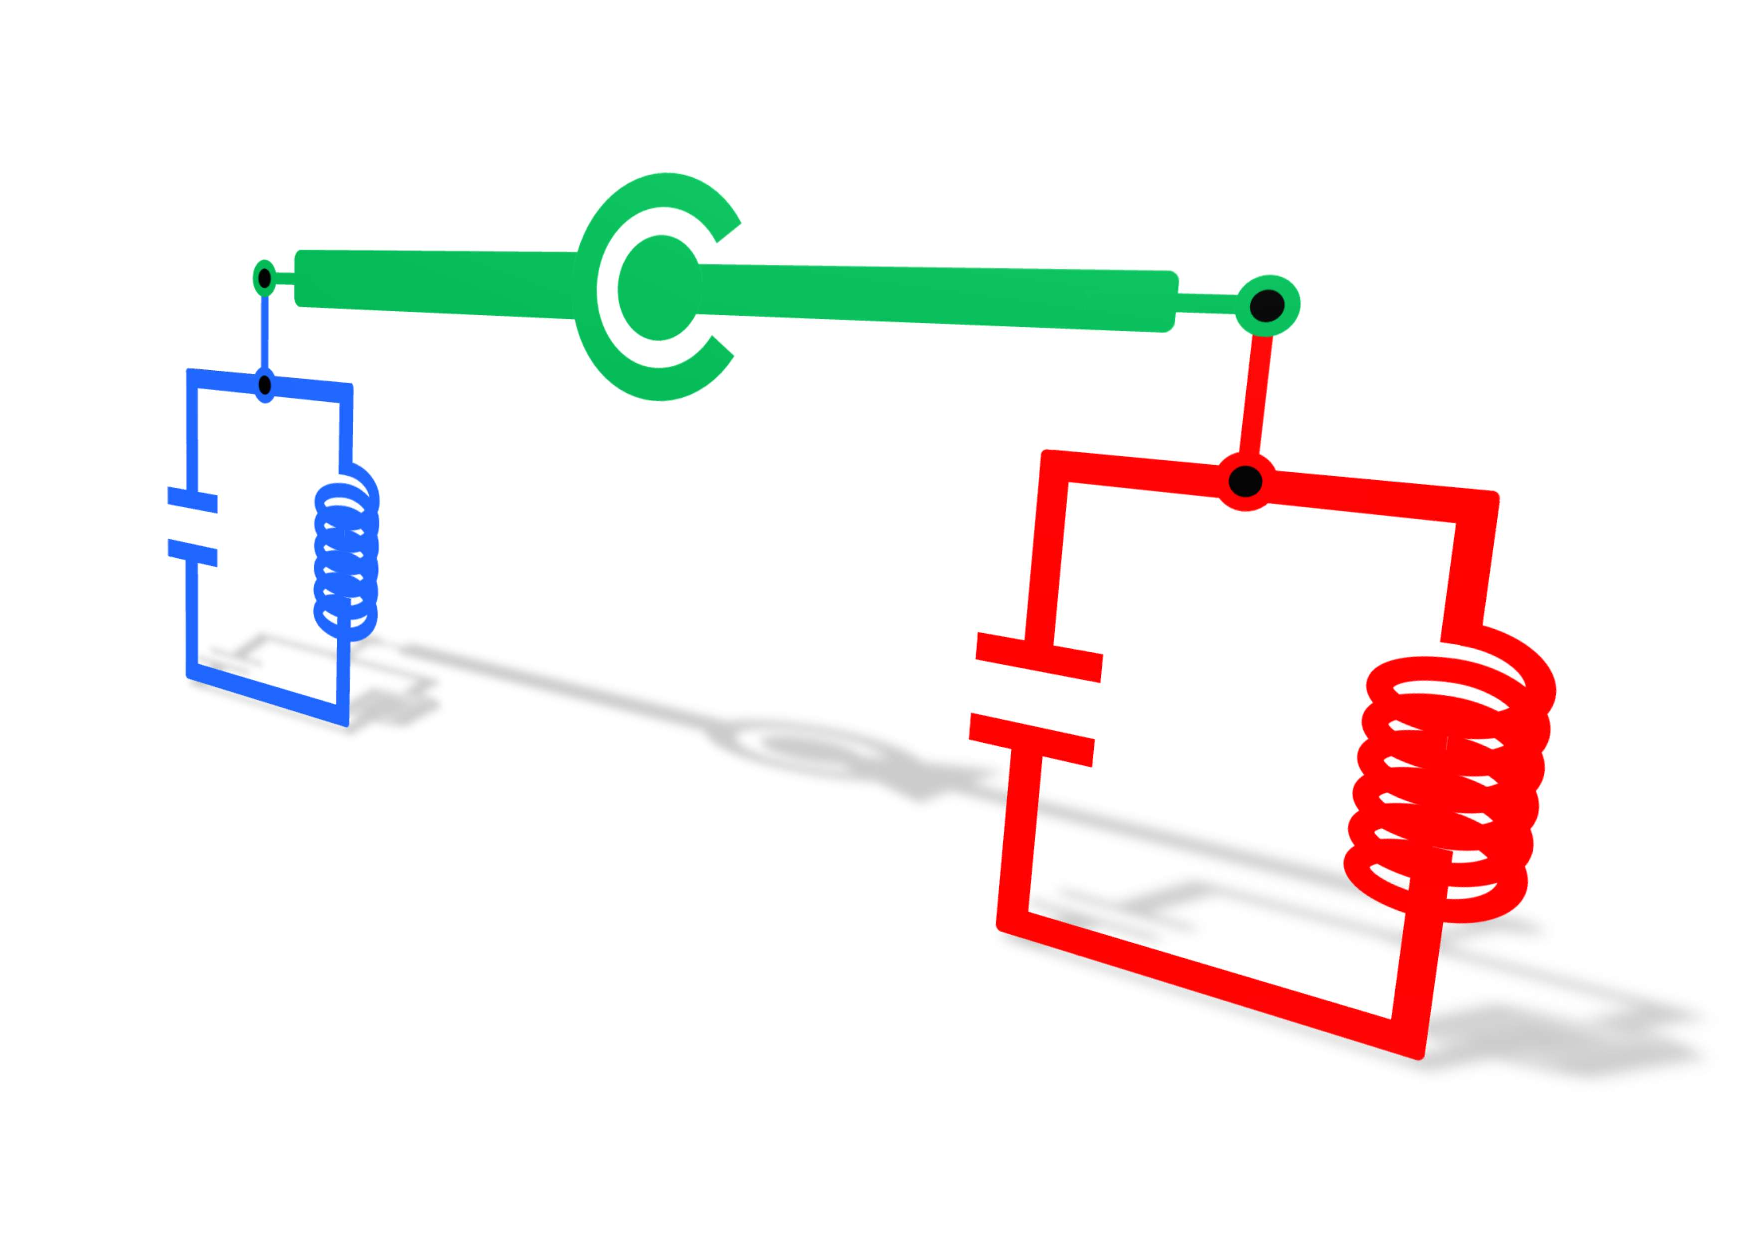
\includegraphics[width=16cm]{表紙2.pdf}
        \end{figure}
        {\Large \today}\\
        \vspace{10truept}
        {\Large 東京理科大学大学院 理学研究科物理学専攻 蔡研究室\\
        (学籍番号 1219537)}\\
        \vspace{20truept}
        {\huge 宮永 崇史}\\

    \end{center}
\end{titlepage}
%\maketitle
%\frontmatter
\addcontentsline{toc}{chapter}{序章}

\section*{序章}
超伝導体を用いた擬似人工原子システムの確立\cite*{nakamura1999coherent}から約23年を経た現在、超伝導量子計算機の開発に注目が集まっている。量子計算機が古典コンピュータと比較して有意な結果を発揮するためには約100万もの擬似人口原子(以下量子ビット)を集積してからだといわれており、回路の集積度は年々増加している。
回路に装填される素子は量子ビットだけではない。量子情報を取得する読み出し素子。量子ビット同士を相互作用させる結合素子。量子情報を伝送させる伝送ライン。これら素子群をパッケージングする回路デザインも量子ビットの集積度に大きく寄与する。当研究室でも万能型量子計算機、専門特化型量子計算機の回路アーキテクチャをそれぞれ提案しており、2次元平面状で実装可能であることが利点である。
\setcounter{tocdepth}{2}
\tableofcontents
%\mainmatter

\chapter{序章}
    \begin{abstract}
        研究の目的
    \end{abstract}
    \section{超伝導回路の大規模化}
    本研究の目的は共振器間の高強度結合素子の開発である。まずはこの研究のモチベーションについて説明することから始める。
    序章でも述べたが超伝導量子回路の集積度は年々向上しており、知名度の高い企業が研究開発に乗り出していることからも世間からの注目度は非常に高い。しかしながら、各々の量子ビットを効率よく相互作用させようとする際にはまだまだ課題も多い。超伝導量子回路を用いた大規模な集積回路として有名なのはD-wave社の量子アニーリング回路、Googleの万能型量子回路であるがその2つの例を見ても各々の量子ビットの全結合は実現できていない。量子ビットと結合素子を直接結合させるには回路デザインの観点から限界が生じている。我々の研究チームでは量子アニーリング型及び万能型のそれぞれについて2次元回路アーキテクチャの開発に取り組んでいる。この2つのアーキテクチャのうち特に量子アニーリング回路では本稿のテーマである。共振器間の高強度結合素子の開発が要となる。以下に大規模アニーリング回路を駆動するために必要なここの超伝導素子のパラメータを示す。

    この図には量子ビット間の実質的な結合強度Jijと量子ビットのパラメータが示されている。量子アニーリングはイジンぐモデルを前提に構築されたモデルであり、最終的な解は結合強度Jijにマッピングされる。始状態のパラメータは量子ビットの遷移周波数にマップされるため始状態と終状態において、この2つのパラメータはバランスがとれていることが前提となる。またスイープ時間において突発的な状態遷移を避けるために量子ビットの遷移周波数はGHz帯に設定する必要がある。この状況においてJijの強度をGHz体に保つためには共振器間の結合強度の絶対値には少なくとも400MHzが必要とされる。マッピングの自由度を上げるにはこのJijは正負でのバランスがとれていることが望ましい。
    以上より共振器間の結合に要請される理想的なパラメータは-400MHzから400MHzを自由に変調できるものである。
    先行研究\cite*{Wulschner2016}では-320MHzから37MHzの結合強度を実現しているが、正負両方向において強度不足であることがわかる。

\section{}

\section{結合振動子}
    本研究のテーマはエンジニアリングな側面が強いが、研究対象としている結合共振回路は物理モデルとしても非常に興味深い内容である。量子力学と古典力学のアナロジーとして連成振動子モデルは多くの研究がなされている。\cite*{Rodriguez2016}\cite*{Ivakhnenko2018}\cite*{Novotny2010}
    上記のモデルは一般的な共振素子(振動子)と共振素子を結合した系を理論的視点から論じている。今回作成した共振回路は共振器間のダイレクトな結合強度を変調できるという点で非常に魅力的である。一般的な共振素子はその遷移周波数がすべて同一であり、共振回路の周波数を持った光子を外部から入力しても高準位へと遷移してしまい、光子の放出現象は示さない。しかし、振動子間に結合項が存在すると振る舞いは一変し新たな固有モードが出現する。古典力学ではしばしばこのモードのことを基準モードと呼んでいる。こ


\chapter{原理}
    \begin{abstract}
        超伝導回路の紹介と結合素子の物理モデルの導入
    \end{abstract}
    \section{物理モデル}

\section{超伝導回路素子}

    \subsection{超伝導共振器}

        \subsubsection{超伝導分布定数回路}

        \subsubsection{超伝導準集中定数回路}

    \subsection{ジョセフソン接合}

    \subsection{rf-SQUID}

    \subsection{dc-SQUID}

    \subsection{カイネティックインダクタンス}
    
    \subsection{ミアンダインダクタンス}


\chapter{実装}
    \begin{abstract}
        結合素子の設計手法と作成方法を解説する。第1節では本研究で作成したサンプルを時間軸に沿って初期サンプル、中期サンプル、後期サンプルとして区別した。諸所のサンプルに施した工夫についても定量的な解説を加えた。
    \end{abstract}
    \section{設計}
        今回測定したサンプルは3つである。作成時期順に列挙すると、基本形となるrf-SQUIDを共振器間に配置したLCC。そしてrf-SQUIDと共振器間の結合部にジョセフソン接合を導入したJLCC、最後に接合部をミアンダインダクタンスに変更したMLCCである。まずは基本型の構造は先行論文がとっている手法と全く同じである。
        \begin{figure}[H]
            \centering
            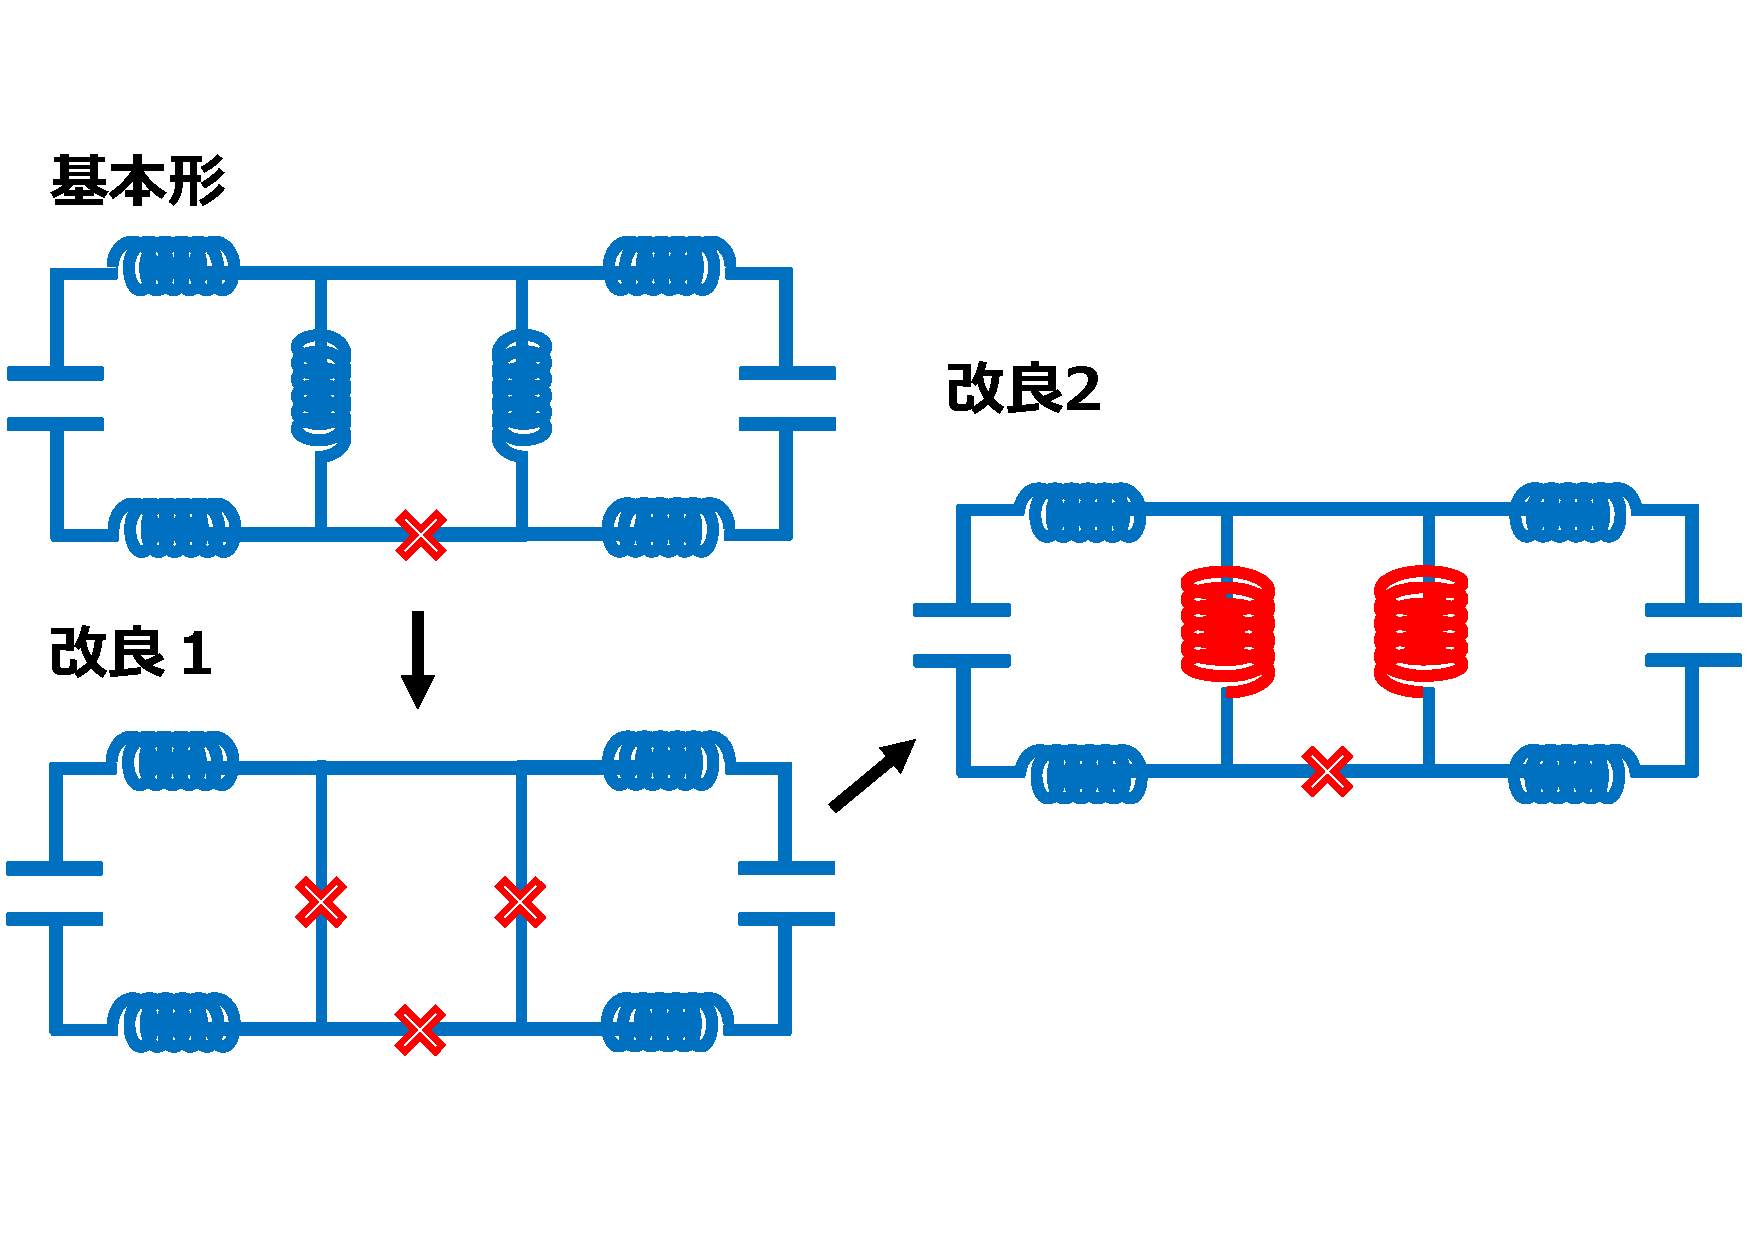
\includegraphics[width=14cm]{sample.pdf}
            \caption{サンプル図}
        \end{figure}
        上図は作成サンプルの回路図を模式的に表したものである。共振器とrf-SQUID間は線路に流れる電流により生じる磁場を介して結合している。模式図のように素子間が完全に接地した状態の結合のことをGalvanic結合と呼ぶ。この構造では、素子間の相互インダクタンスが接地部分の自己インダクタンスとほぼ等しくなるため非常に強力な相互インダクタンスを得ることができる。

        設計のポイントは①rf-SQUID-共振器間の相互インダクタンス増強と②rf-SQUIDスクリーニングパラメータの精密な製造である。この2つのパラメータは結合強度を向上する上で非常に重要な因子となる。
        この2つのパラメータが結合強度向上に大きく寄与するということを基本型であるrf-SQUIDの遷移スペクトルの計算を通して論拠する。
    \subsection{遷移スペクトル計算}
        基本型の回路のハミルトニアンは
        \begin{equation}
            \hat{\mathcal{H}}=\hbar\left(\hat{a}^{\dagger }\ \hat{b}^{\dagger }\right)\left(\begin{array}{cc}
            \tilde{\omega}_{a} & g(\Phi ) \\
            g(\Phi ) & \hat{\omega}_{b}
            \end{array}\right)\left(\begin{array}{l}
            \hat{a} \\
            \hat{b}
            \end{array}\right)
        \end{equation}
        \begin{equation}
            = \hbar \hat{\omega}_{a} \hat{a}^{\dagger} \hat{a}+\hbar \hat{\omega}_{b} \hat{b}^{\dagger} \hat{b}+\hbar g(\Phi)\left(\hat{a}^{\dagger}\hat{b}+\hat{a} \vec{b}^{+}\right)
        \end{equation}

        である。式の前項2つが左右各共振器の調和振動子ポテンシャルである。最終項が結合項であり、この結合項に依存して2つの共振器が反発することを示す。各共振器の生成消滅演算子を
        \begin{equation}
            \hat{c}_{\pm}=\frac{\hat{a} \pm \hat{b}}{\sqrt{2}} \quad \hat{c}_{+}^{\dagger}=\frac{\hat{a}^{\dagger} \pm \hat{b}^{\dagger}}{\sqrt{2}}
        \end{equation}

        と置き換える。ここで演算子$\hat{c}_{\pm}$は各共振器の状態が混合した状態である。このように変換を行うと最終的に得られる状態は
        \begin{equation}
            \hat{H}=\hbar \Omega_+\hat{c}^{\dagger}_+\hat{c}_+ + \hbar \Omega_-\hat{c}^{\dagger}_-\hat{c}_- + \hbar \Delta\left(\hat{c}^{\dagger}_+ \hat{c}_- +\hat{c}^{\dagger}_- \hat{c}_{+}\right)
        \end{equation}

        \begin{equation}
            =\hbar\left(\begin{array}{cc}
            \hat{c}^{\dagger}_{+} & \hat{c}^{\dagger}_-
            \end{array}\right)\left(\begin{array}{cc}
            \Omega_{+} & \Delta \\
            \Delta & \Omega_{-}
            \end{array}\right)\left(\begin{array}{l}
            \hat{c}_{+} \\
            \hat{c}_{-}
            \end{array}\right)
        \end{equation}

        となる。この時$\Omega_+ = (\omega_a+\omega_b)/2 + g$、$\Omega_- = (\omega_a+\omega_b)/2 - g$、$\Delta = (\omega_a-\omega_b)/2$である。これより、2つの独立な調和振動子系は結合項$g$によって新たな基準モードで書き表すことができる。この新たな基底同士は元々の共振周波数の離調$(\omega_a-\omega_b)/2$で書き表すことができる。また変換前の基底、つまり左右の調和振動系の結合項$g$は新基底において新固有値の差分に現れる。これを図示すると以下のようになる。
        \begin{figure}[H]
            \centering
            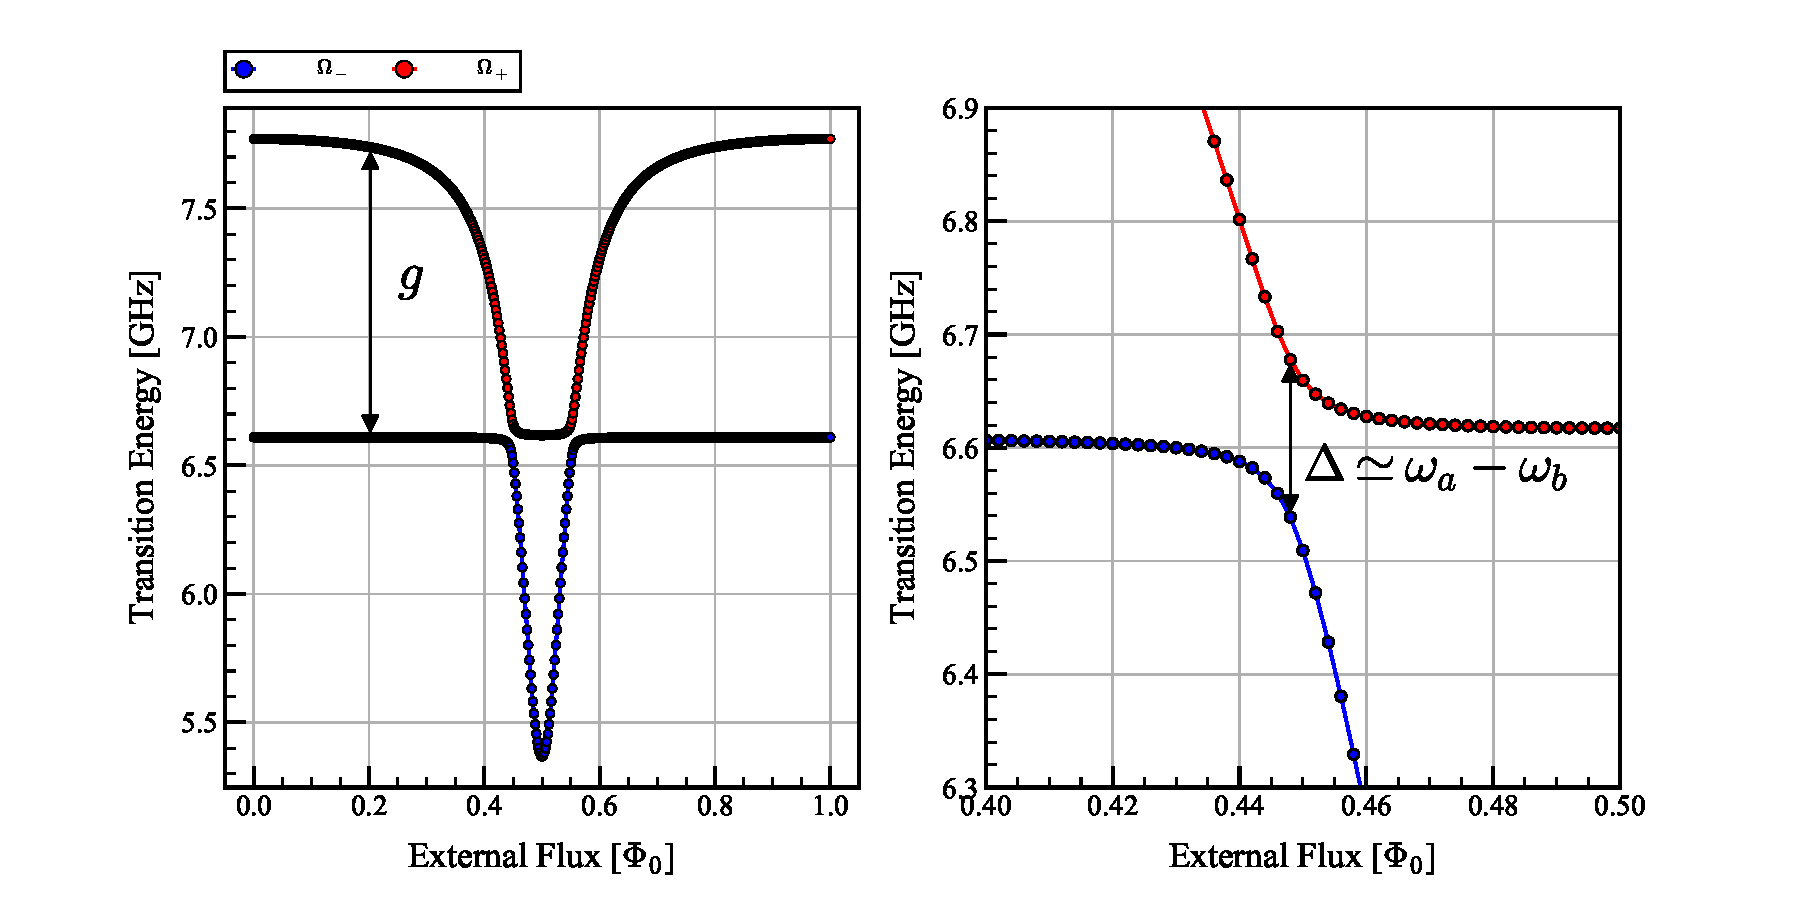
\includegraphics[width=16cm]{standard_eigen.pdf}
            \caption{遷移周波数図}
        \end{figure}
        つまり、測定において得られた2つの基準モードの差分を計算することにより元のハミルトニアンの結合強度gを見積もることができる。以下に上図に対応する外部磁束に対応する結合強度の図をプロットする。
        \begin{figure}[H]
            \centering
            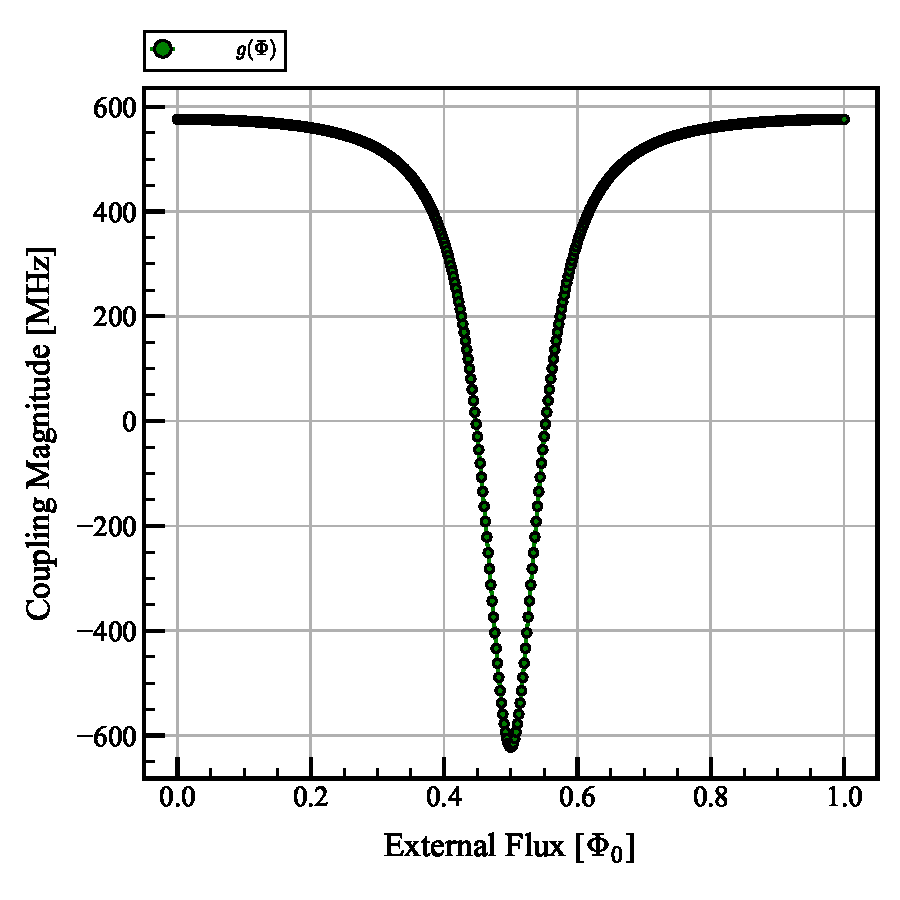
\includegraphics[width=7cm]{standard_coupling.pdf}
            \caption{結合強度図}
        \end{figure}

        既に述べたように今回作成した結合回路において強度をドメスティックに変えるパラメータはrf-SQUIDのスクリーニングパラメータとrf-SQUIDと共振器間の相互インダクタンスである。それぞれのパラメータを変えた時にどのように結合強度が変化するのを示した図が以下である。
        \begin{figure}[H]
            \centering
            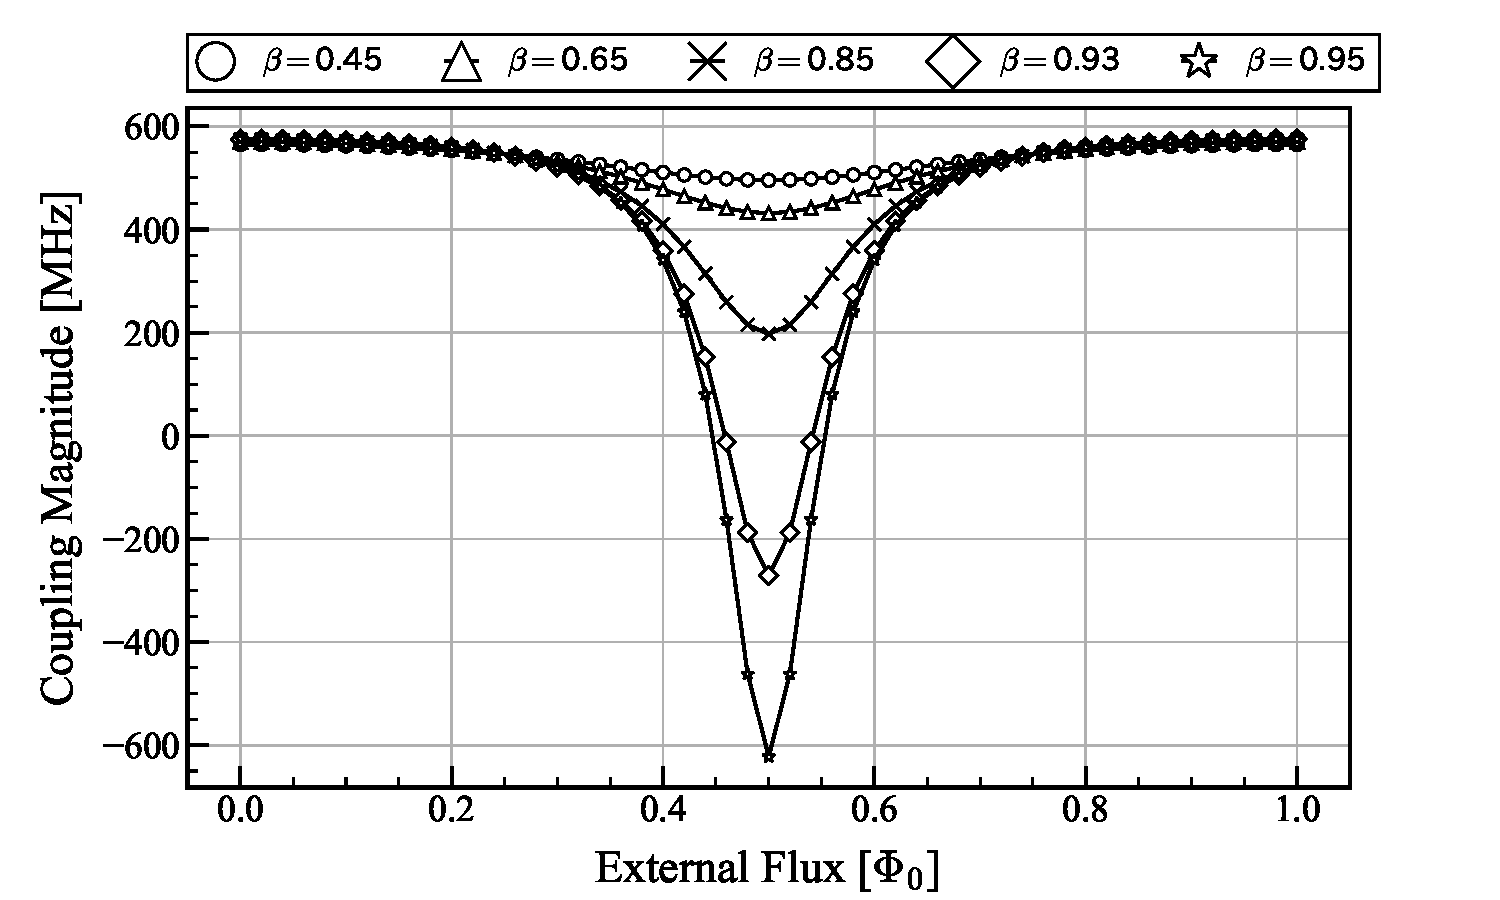
\includegraphics[width=12cm]{standard_coupling_beta.pdf}
            \caption{結合強度の$\beta$依存性}
        \end{figure}
        また、外部磁束を0.5に固定子、$\beta$の値のみを変更することによる結合強度の対応をプロットすると$\beta$が0.8を超えたあたりで急激に結合強度が変化していることがわかる。
        \begin{figure}[H]
            \centering
            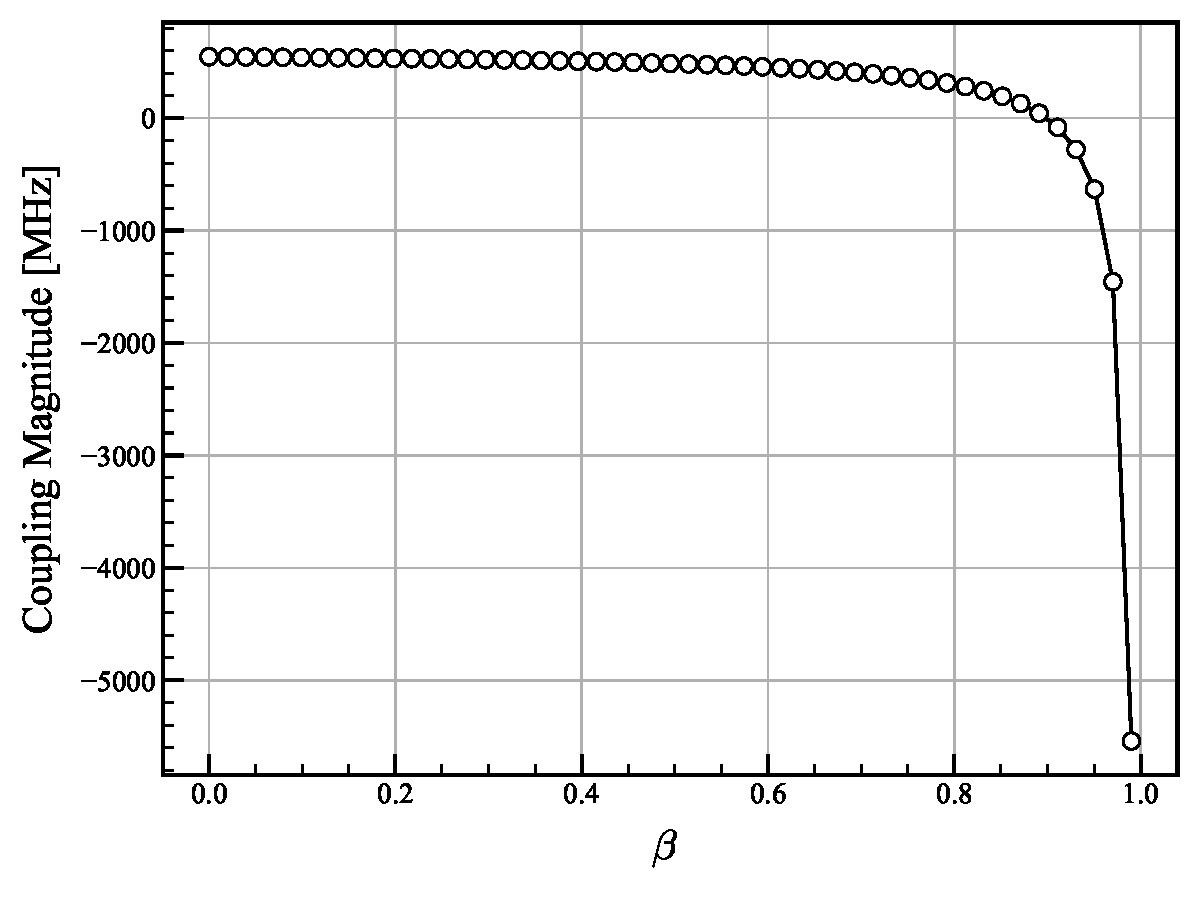
\includegraphics[width=8.5cm]{standard_coupling_betasweep.pdf}
            \caption{結合強度の$\beta$依存性}
        \end{figure}
        スクリーニングパラメータが1を超えるとこの関数は発散してしまうため、最適な動作点としては$0.8<\beta<0.95$付近が妥当であると考えられる。しかしながら、後述するが実際にはスクリーニングパラメータをこの領域内に収めることは非常に困難である。
        スクリーニングパラメータはジョセフソンインダクタンス$Lj$とrf-SQUIDのループインダクタンスLsにより$\beta=Ls/Lj$と表現されるが仮にLsの値を0.224[nH]で設計した場合
        \begin{equation*}
            L_{jdes} = 0.258 \pm 0.022\ [nH]
        \end{equation*}
        経験的にジョセフソン接合の作成にはインダクタンスにしてOOnHのばらつきが出るため、再現性が非常に低くなる。
        そこで、今回作成したサンプルには単一ジョセフソン接合の代替にdc-SQUIDを用いた。
        \subsection{$\beta$ ループによる変調}
        dc-SQUIDはジョセフソン接合2つを含んだ超伝導ループであり、この超伝導線路のインダクタンスは実効的に
        \begin{equation*}
            L_{jsq} = \frac{\Phi_0}{4\pi I_c|\cos(\pi(\frac{\Phi_{ext}}{\Phi_0}))|}
        \end{equation*}
        である。
        \begin{figure}[H]
            \centering
            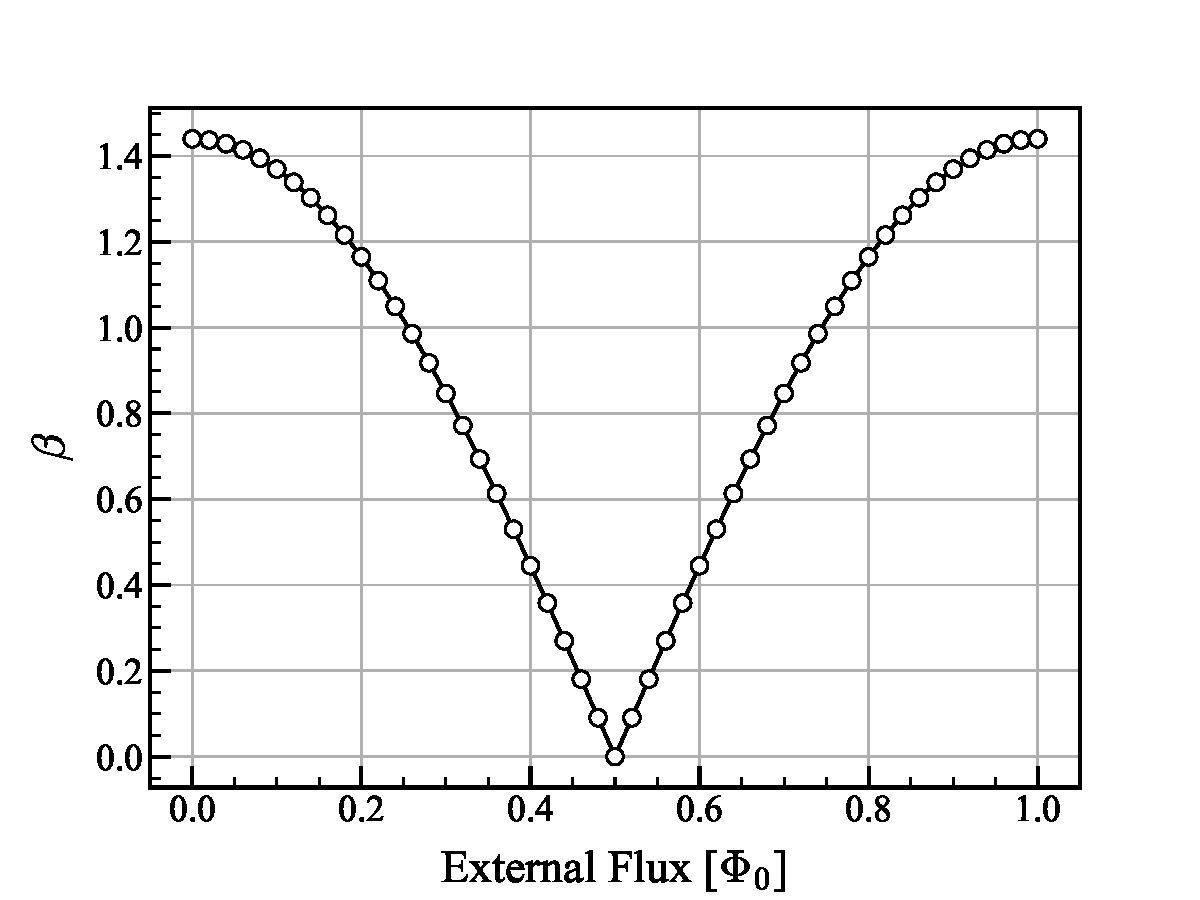
\includegraphics[width=8.5cm]{dc-squid.pdf}
            \caption{dc-SQUIDによる$\beta$変調}
        \end{figure}
        この素子によりrf-SQUIDのジョセフソンインダクタンスを外部磁束によって変調することが可能となった。
        次にrf-SQUIDと共振器間の相互インダクタンスを向上させる手法について考える。
        今回採用した方法はミアンダインダクタンスを用いたものである。ミアンダインダクタンスは細線を蛇行させることにより各線路の相互インダクタンス、単純な線路長の増加によりインダクタンスを線路エリアに対して大きくすることができる。この設計において相互インダクタンスに注目することとなった経緯を説明する。
        修士の研究において大別して3種類のデバイスを測定したと述べたがこのうちJLCCの結果を受けてである。このサンプルはジョセフソン接合をrf-SQUIDと共振器間に挿入することで、ジョセフソンインダクタンスを用いて相互インダクタンスを強める目的で導入した。結果として望むような成果は得られなかったが次の2つの収穫が得られた。

        ①正方向の結合強度を向上する手段として相互インダクタンスの寄与は非常に大きいこと。
        
        ②相互インダクタンスはその大きさの2乗によって結合強度を増強すること。
        
        スクリーニングパラメータ$\beta$の精密な操作が結合強度を急激に増加させることは既に述べたが、結合素子として扱う際には磁束の急激な変化は望ましくない。操作が困難になることはもちろん急激な値の変化は解析をするさいにも困難を要する。そこで、まずは相互インダクタンスで可能な限りな結合強度の増強を試みる。
        また、共振器間の1次結合(直接的な相互インダクタンスを強めるためにrf-SQUIDの構造も縦長なループ構造へと修正した。
        \begin{figure}[H]
            \centering
            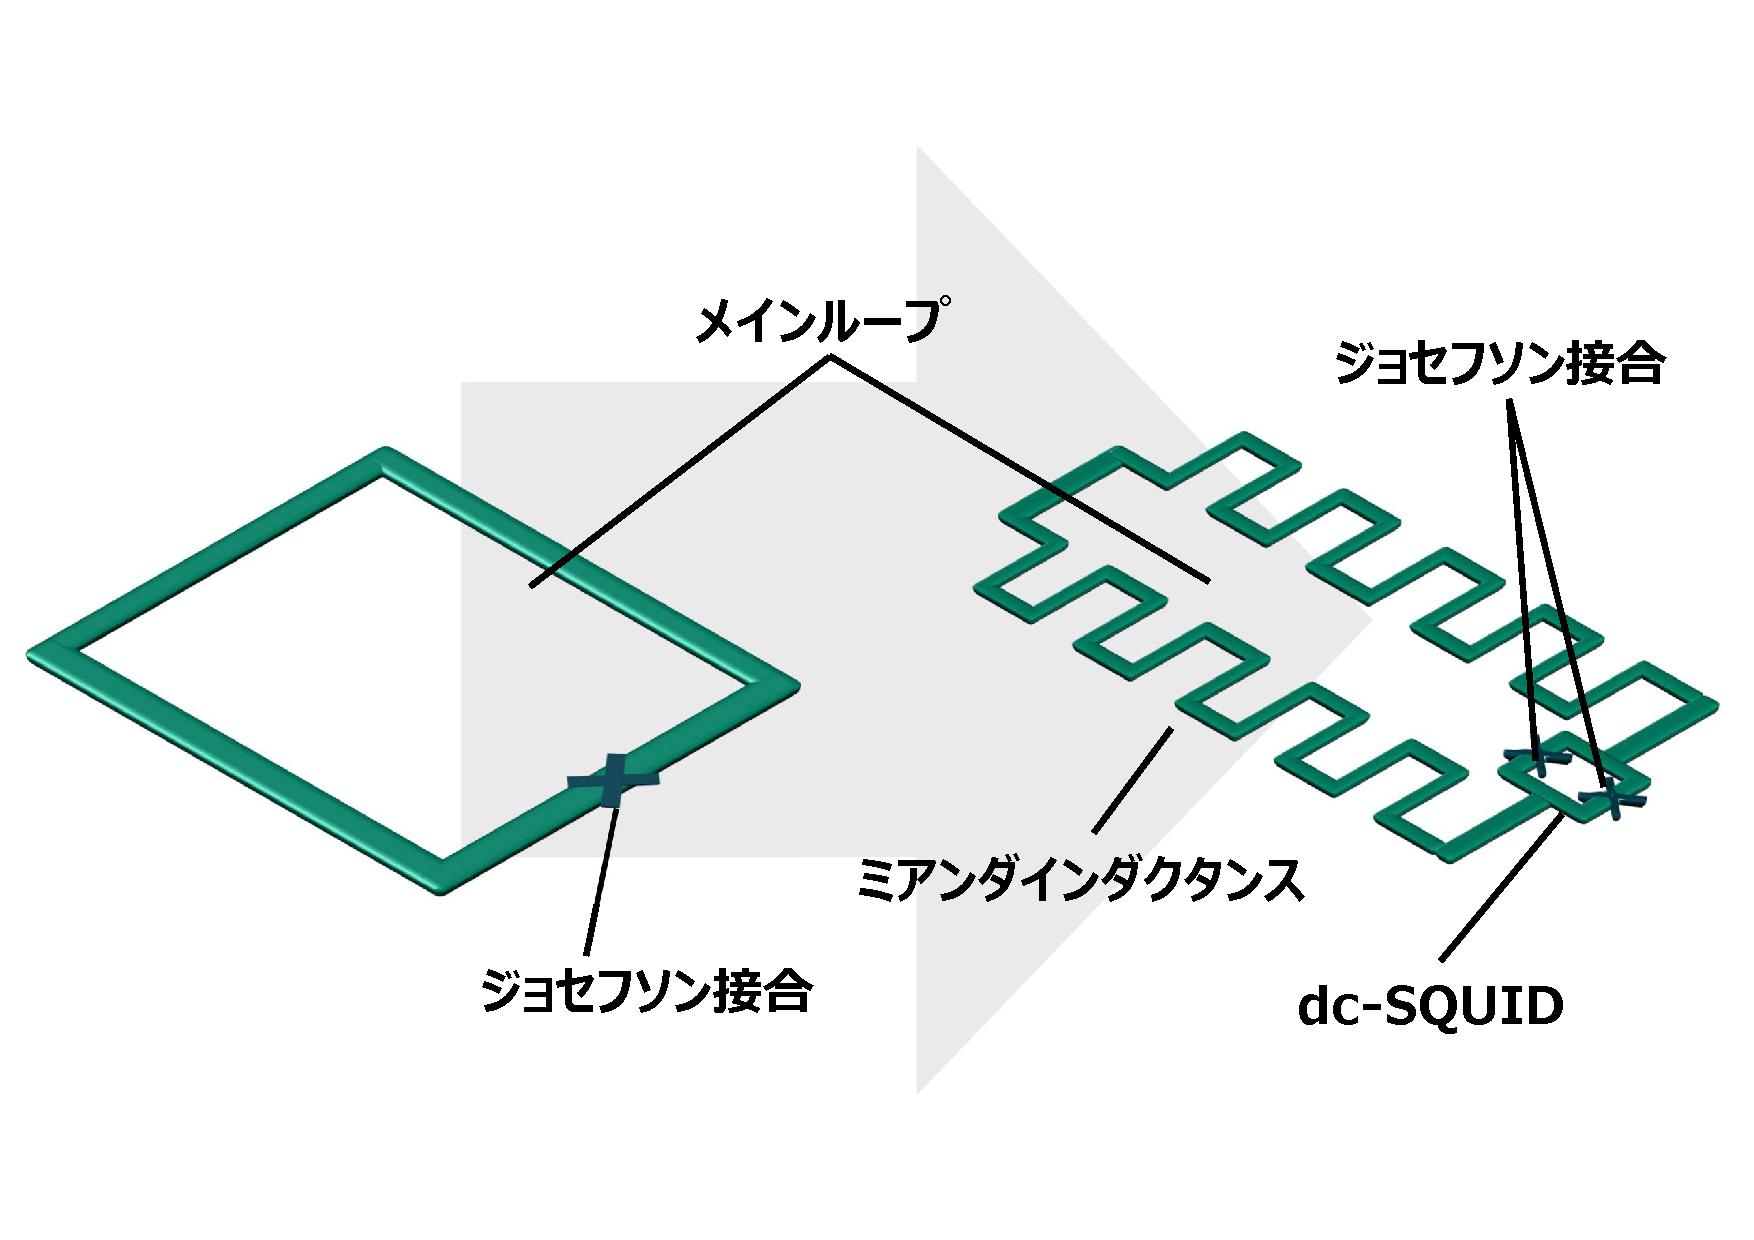
\includegraphics[width=12cm]{samplefigure.pdf}
            \caption{aMLCCの模式図}
        \end{figure}
        次に配線構造を考える。サンプル上に載せる配線の本数は少なければ少ないほどに良い。特に磁束バイアスを用いる場合、クロストークを考慮する必要がある。今回のサンプルでは少なくとも2つの独立な電流源が必要となる。1つはdc-SQUIDにバイアスしてスクリーニングパラメータを調整する電流源、もう一つがrf-SQUIDのメインループを貫き、結合素子の強度を変更するための磁束バイアスである。ここでは配線構造について考える。
        実験環境ではサンプル上に載せるオンチップバイアスラインとサンプルをマウントするサンプルホルダー上に積載しているグローバルフラックスを用いることができる。配線本数を減らすという観点ではこのグローバルフラックスを利用するのが好ましい。しかしながら、グローバルフラックスはサンプル全体に均一な磁場がかかるため、メインループとdc-SQUIDのループ面積比を極端に差別化することで独立な操作がしやすいように工夫した。
        \begin{figure}[H]
            \centering
            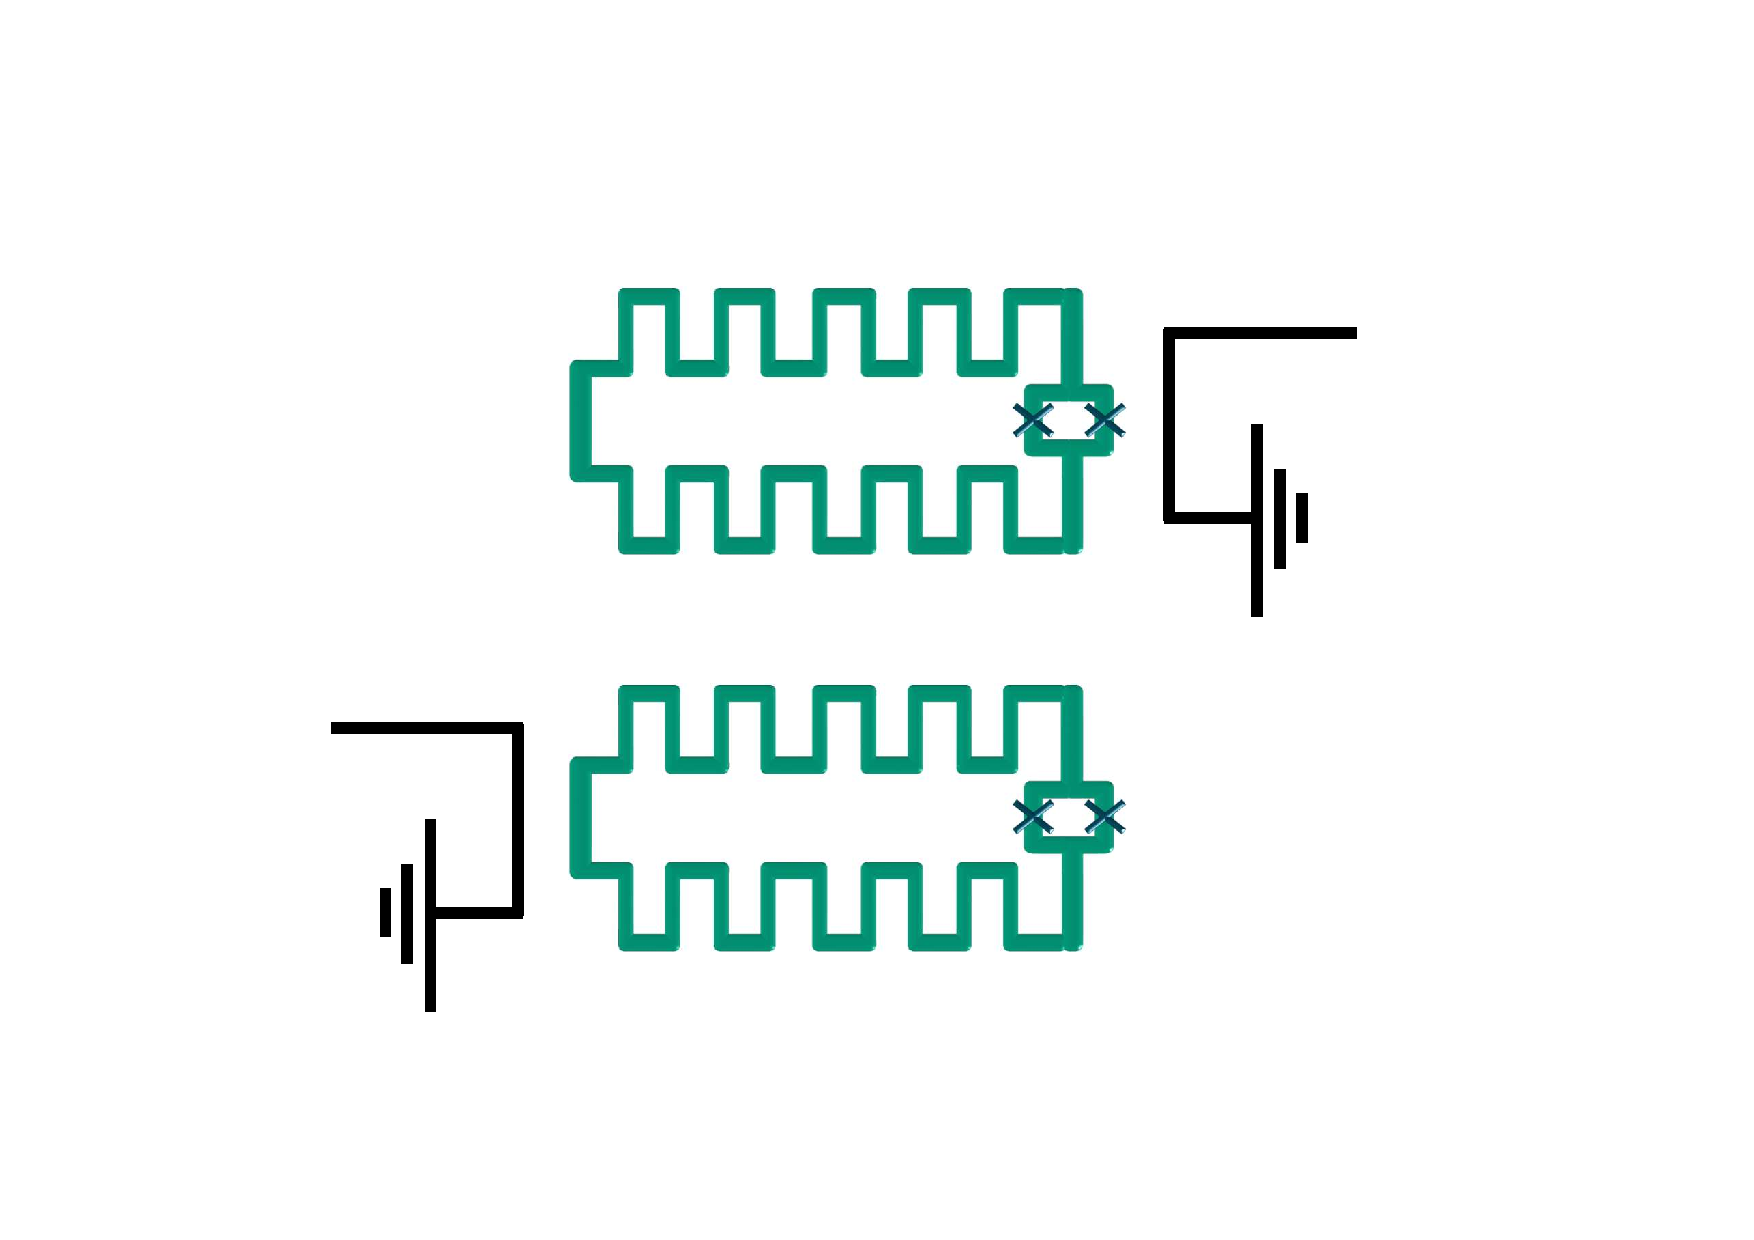
\includegraphics[width=10cm]{配線.pdf}
            \caption{aMLCCの模式図}
        \end{figure}
        一方をグローバルフラックスで駆動し、もう一方をオンチップバイアスで駆動することを考える場合、配線の仕方は上記図のような2つの方法が考えられる。今回はメインループ側にオンチップバイアスを取り付けた。グローバルバイアスを全体に印加しているためメインループ、dc-SQUIDを均一磁場が貫く。貫く磁束量子の本数はループの面積比に依存するため、メインループの面積比をdc-SQUIDの100倍にすることで差別化した。まずは上部の配線構造について説明を加えるとこの配線構造ではグローバルバイアスでrf-SQUIDを貫く磁束を固定した上で新たにオンチップバイアスでdc-SQUIDに磁束を印加することでrf-SQUIDのスクリーニングパラメータを調整することができる。この配線構造で問題となるのはオンチップバイアスラインとrf-SQUIDのメインループが非常に近接しているということである。クロストークを可能な限り抑制することを考えるとこの配線は望ましくない。
        次に下部の配線構造であるが、この場合ではグローババイアスでdc-SQUIDを貫く磁束を固定した上でrf-SQUIDを貫く磁束をオンチップバイアスで調節することを目的としている。この場合オンチップバイアスがdc-SQUIDに影響するクロストークは非常に小さいといえる。ループの形状を縦長にするという工夫はクロストークを抑制するという点でも非常に合理的であることがわかる。しかし、クロストークがいかに小さいとはいえ、オンチップバイアスからdc-SQUIDに寄与するクロストークは少なからず存在する。測定を行う際にはそれぞれの電流源がそれぞれのループに寄与するクロストークをインダクタンス行列を用いて評価する。

    \subsection{共振器}
        共振器には超伝導準集中定数素子を用いた。超伝導量子回路で一般的に使用されているCPW型共振器はグランドと伝送線路の距離を伝送損失の少ない50$\Omega$で保つことで単位長さあたりのキャパシタンス$Cp.u.l$とインダクタンス$Lp.u.l.$を求め、伝送線路の長さを乗じることで回路全体のキャパシタンスとインダクタンスを決定している。非常にこの構造は伝送損失が少なく非常に簡便に共振器の設計ができる点がメリットとなる。他方で単位長さあたりのキャパシタンスとインダクタンスが一定にするため複雑な構造をつ繰り出すことはできない。また集中定数回路のように局所的に共振パラメータを調節することには向かないといえる。他方で今回採用した準集中定数型の共振器は意図的に局所的なキャパシタンスとインダクタンスを設けることでLC共振器をつくり出している。この場合共振周波数は回路の局所的な共振パラメータにより求まり、線路長には依らない。
        共振器のパラメータ計算には手計算に依る解析的な方法と電磁界シミュレーションに依る2つの方法を用いた。電磁界シミュレーションにはAWR社のマイクロウェーブオフィス(ver14.03)を使用した。
    \subsection{電磁界シミュレーション}
        共振器の1次結合は電磁界シミュレータ―を用いて算出した。シミュレーションした構造は以下の2つである。
        \begin{figure}[H]
            \subfigure{
            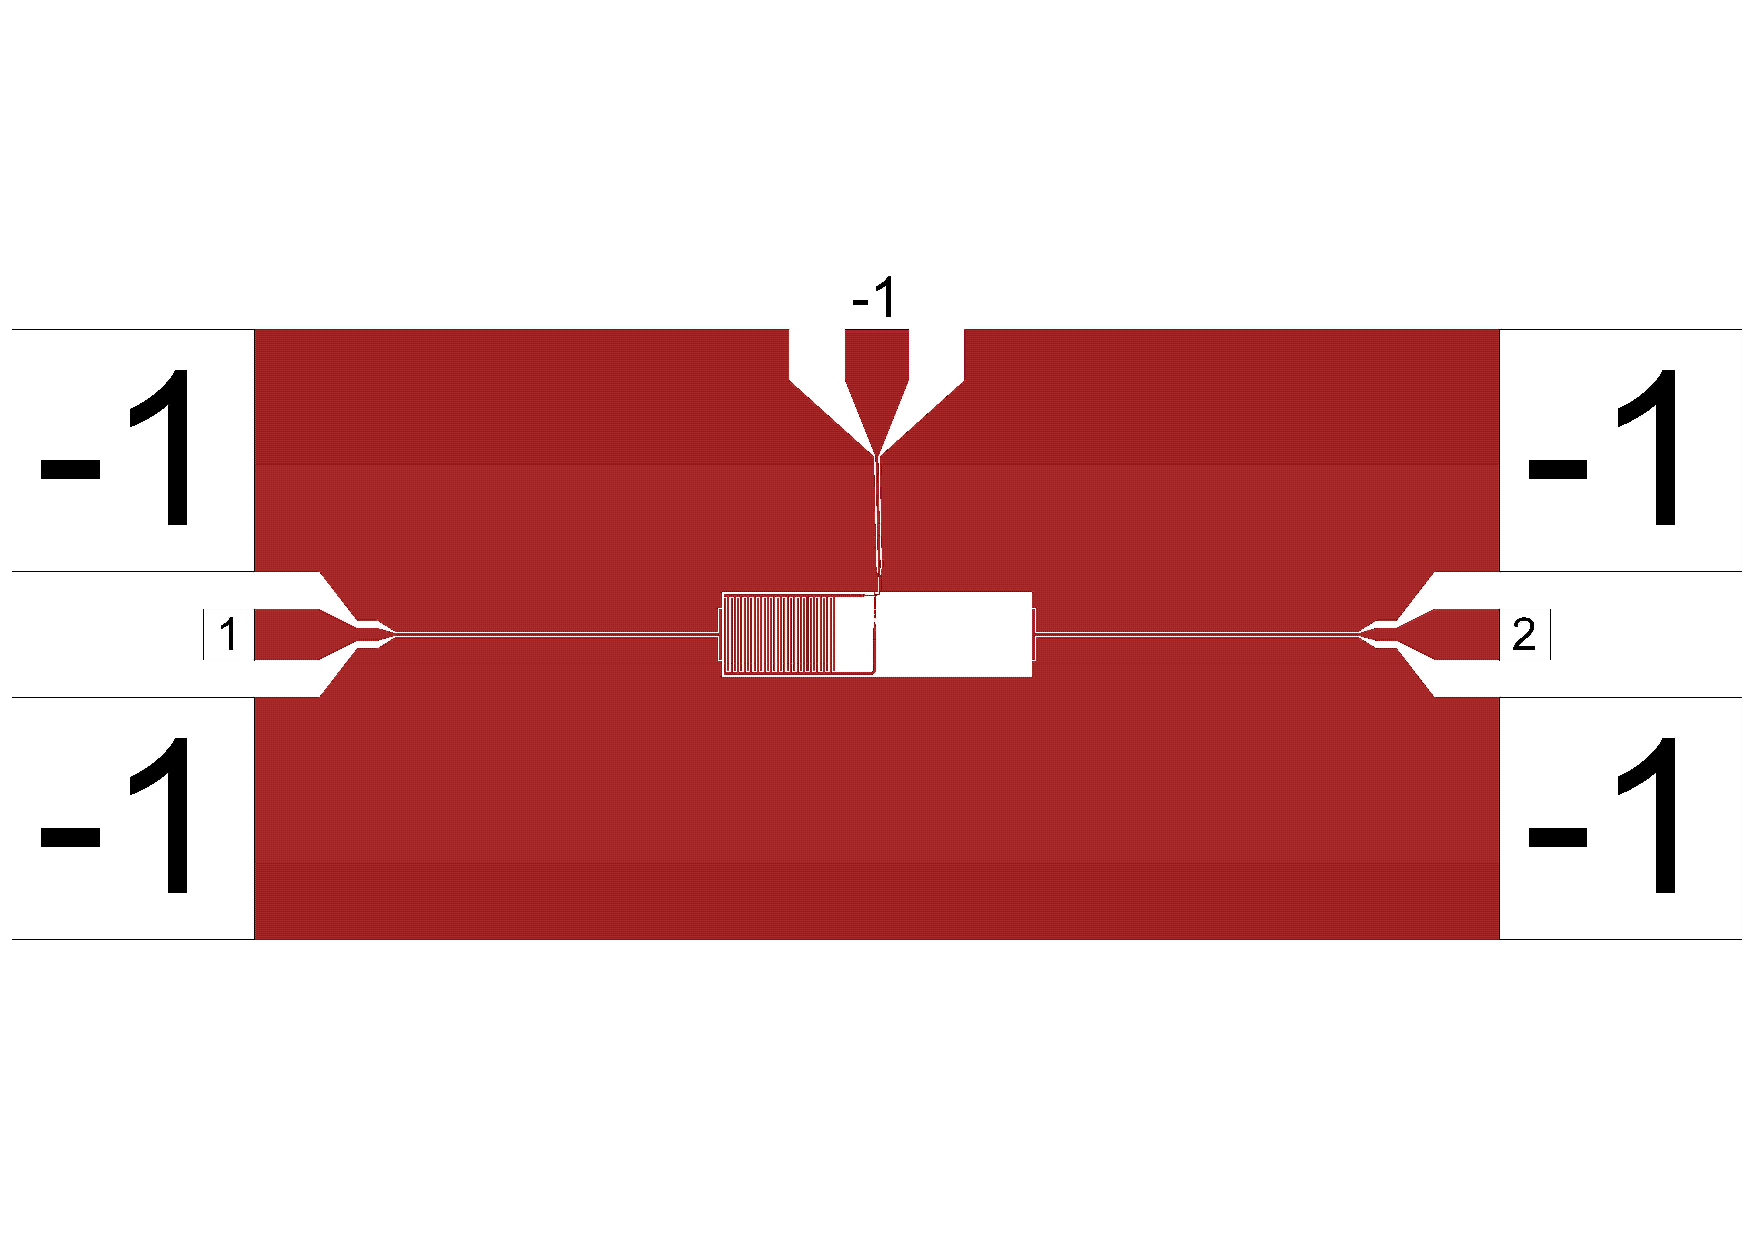
\includegraphics[width=0.5\columnwidth]{resonator_design_for_mwo.pdf}
            }
            \subfigure{
            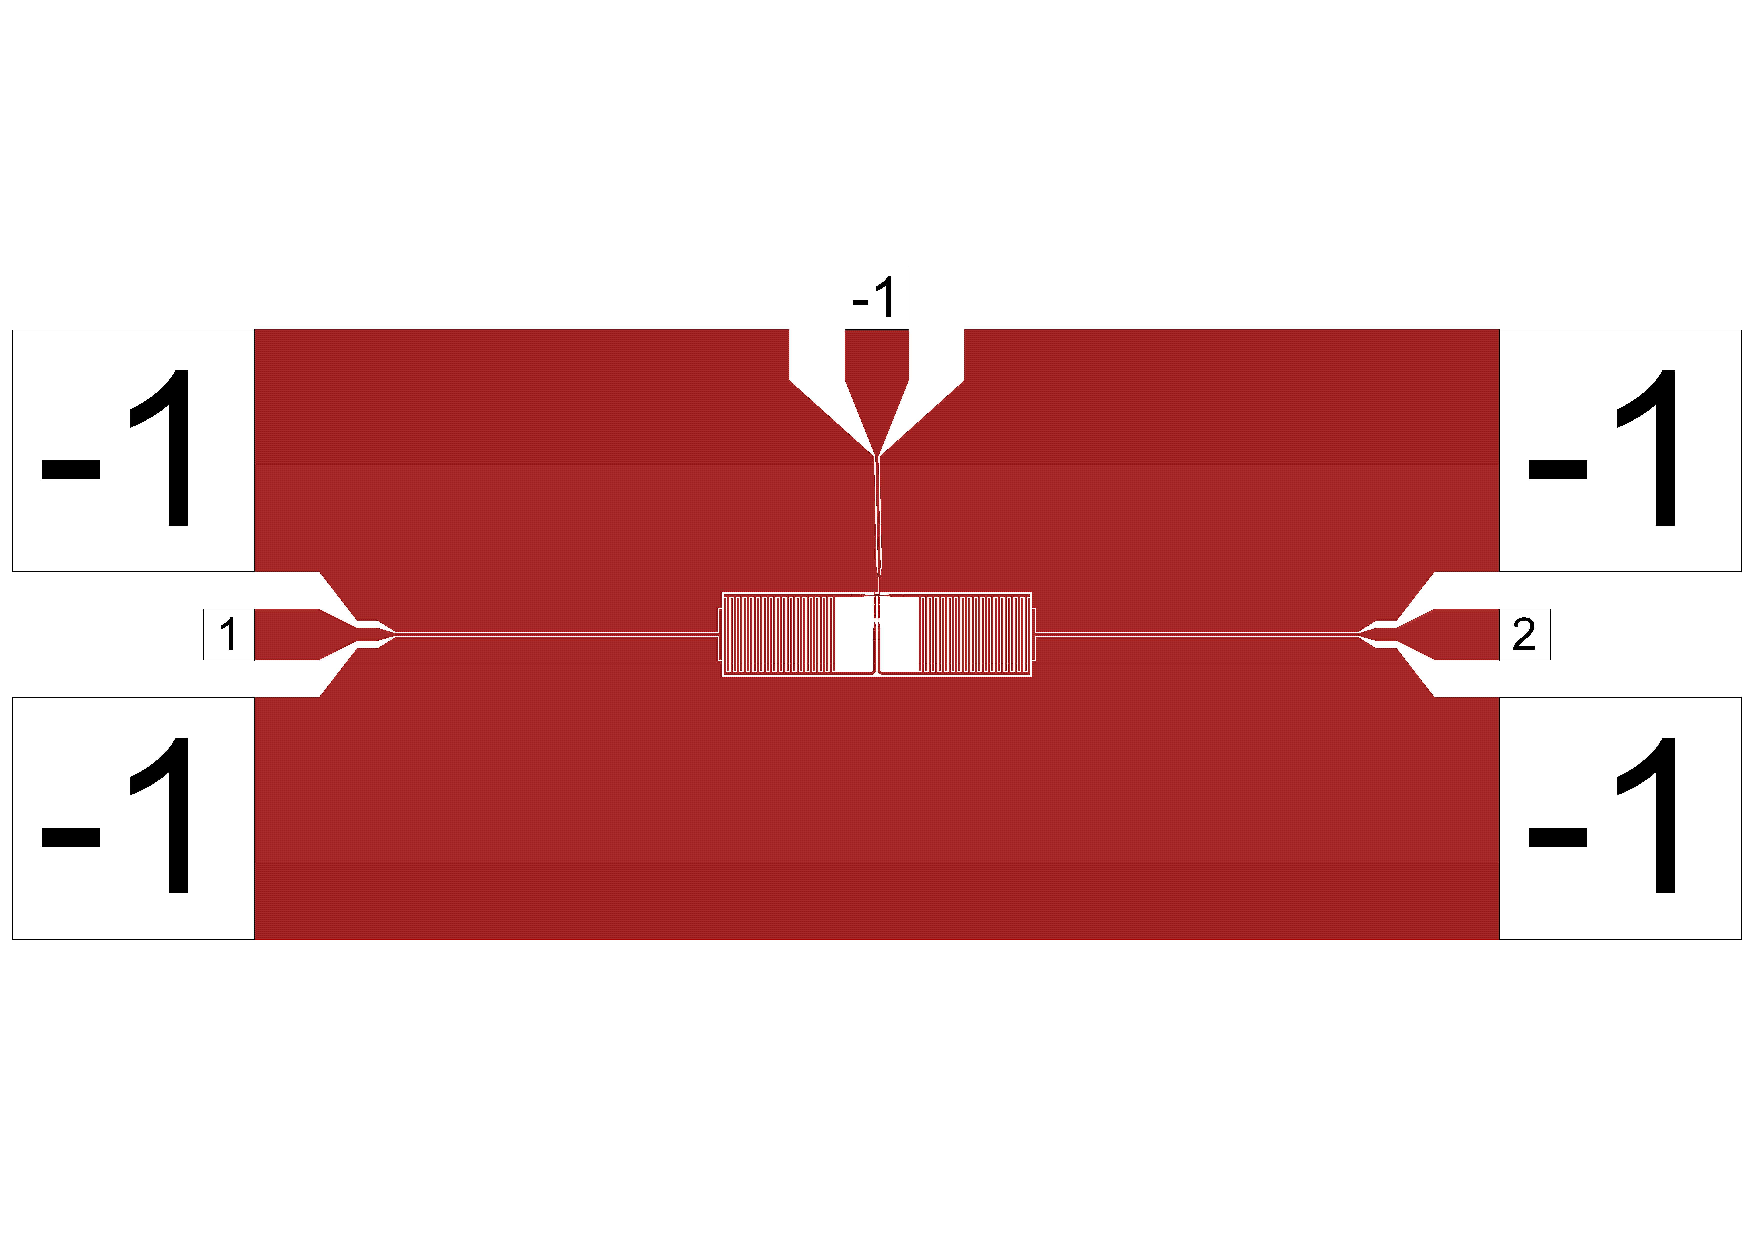
\includegraphics[width=0.5\columnwidth]{coupled_resonator_mwo.pdf}
            }
            \caption{電磁界シミュレーションに使用した構造}
        \end{figure}
        図中右側の構造は左の構造を左右対象に配置したものである。すなわち共振周波数は左右の共振器で同一になっている。この構造を電磁界シミュレーションすると図中左の構造物をBare Resonaotr図中右側の構造物を左からResonator A、Resonator Bと表現する。Resonator AとResonator BはBare Resonatorを中点としてそれぞれ結合強度の1/2で反発することが予想される。このシミュレーションによってもっと待った共振周波数の差は共振器間の1次結合gに対応する。
        \begin{figure}[H]
            \centering
            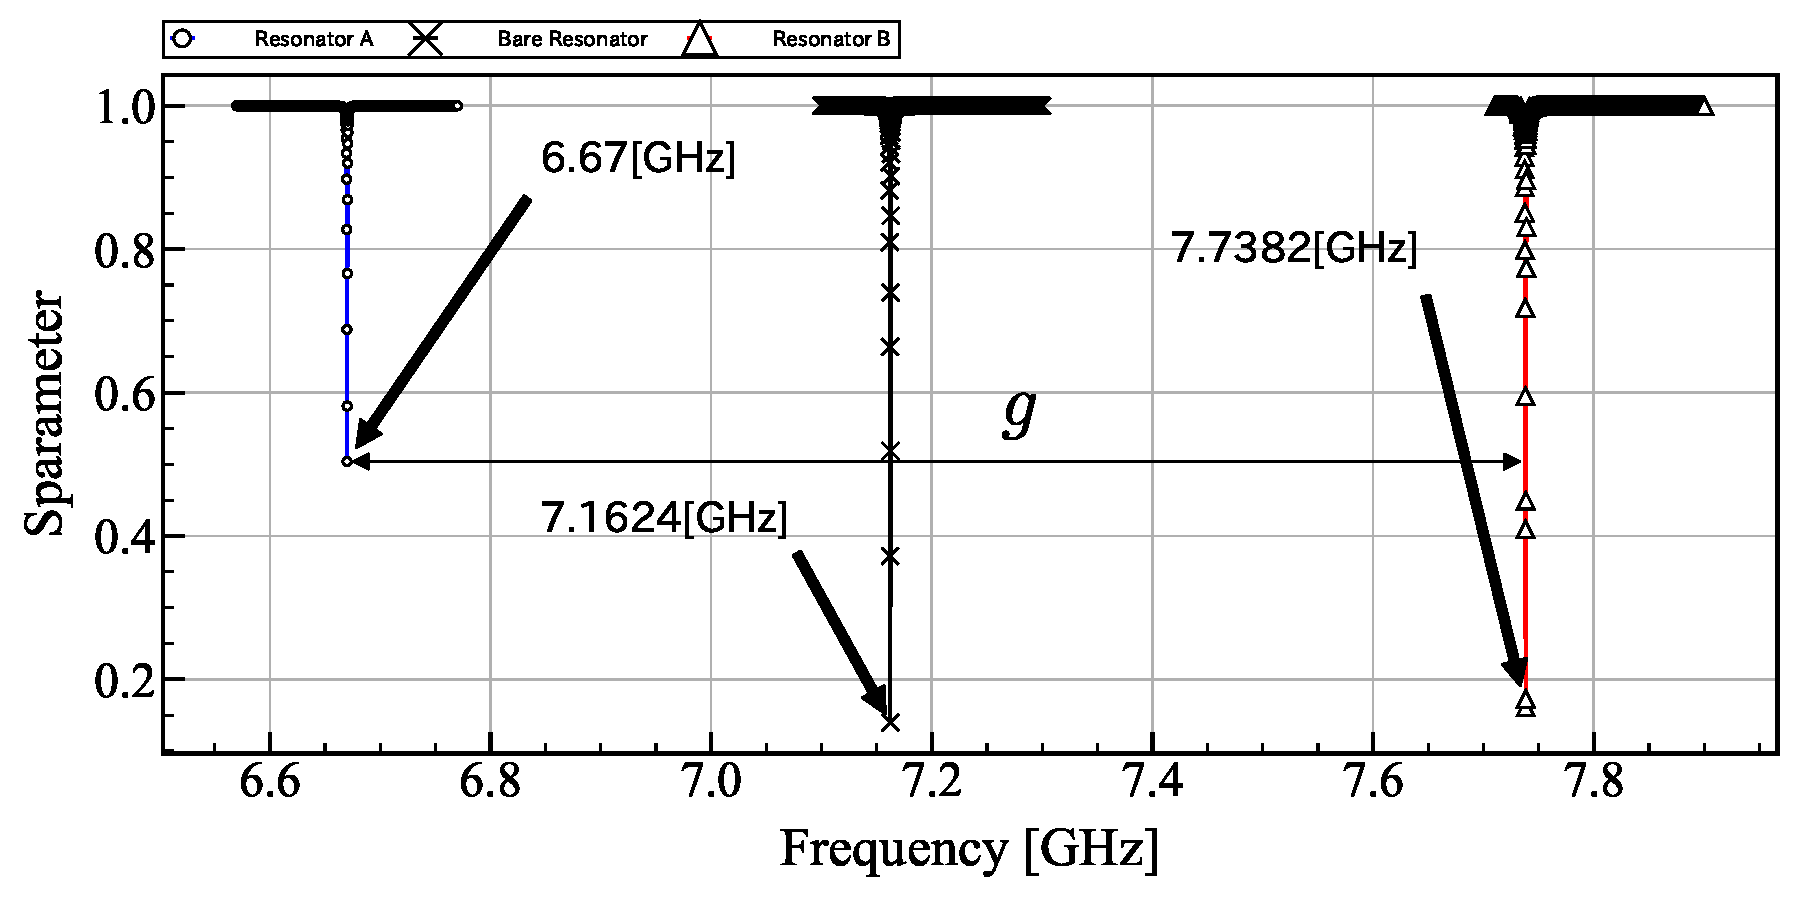
\includegraphics[width=14cm]{mwo.pdf}
            \caption{dc-SQUIDによる$\beta$変調}
        \end{figure}
        構造が同じ共振器間に結合強度gが存在する場合、共振器は結合強度に依存して反発する。これは電気回路からも求めることができる。補足に詳しい計算を記したので参考されたい。
        電磁界シミュレーションによって算出された共振周波数を以下に示す。
        \begin{table}[h]
            \caption{共振周波数}
            \centering
            \begin{tabular}{@{}cc@{}}
            \toprule
                           & Frequency [GHz] \\ 
                           \hline \hline
            Resonator A    & 6.6700          \\
            Resonaotor B   & 7.7382          \\
            Bare Resonator & 7.1624          \\ \bottomrule
            \end{tabular}
            \end{table}
        また、同時に各共振器に流れるゼロポイントフィールド電流$I_{ZPF}$は及び結合強度、相互インダクタンスについては
        \begin{table}[h]
            \caption{結合共振器のパラメータ}
            \centering
            \begin{tabular}{@{}cc@{}}
            \toprule
            Parameter & Value    \\ 
            \hline \hline
            Current        & 5.740 nA \\
            Mutual Inductance       & 0.107 nH \\ 
            coupling constant         & 534 MHz  \\\bottomrule
            
            \end{tabular}
            \end{table}
        次に電磁界シミュレータ―を用いてBare Resonatorのインダクタンスとキャパシタンスを求める。
        図OOについて低周波でのアドミッタンスを求める。低周波、直流源に対してはキャパシタンスがインピーダンスとして強く現れる。この特性を用いてBare Resonatorに置けるキャパシタンスとインダクタンス、特にミアンダインダクタンスの評価をする。
        ミアンダインダクタンスを評価する上で上記のデザインに加えて新たに以下のようなデザインについてもシミュレーションを行った。
\section{製造}

    \subsection{製造パラメータ}

    \subsection{二重角度蒸着}

\section{測定サンプル}

    \subsection{回路パラメータ}


\chapter{測定}
    \begin{abstract}
        本研究の実験環境と冷凍機の冷却原理及び測定の方法について解説する。
    \end{abstract}
    \section{測定環境}
    \begin{figure}[H]
        \centering
        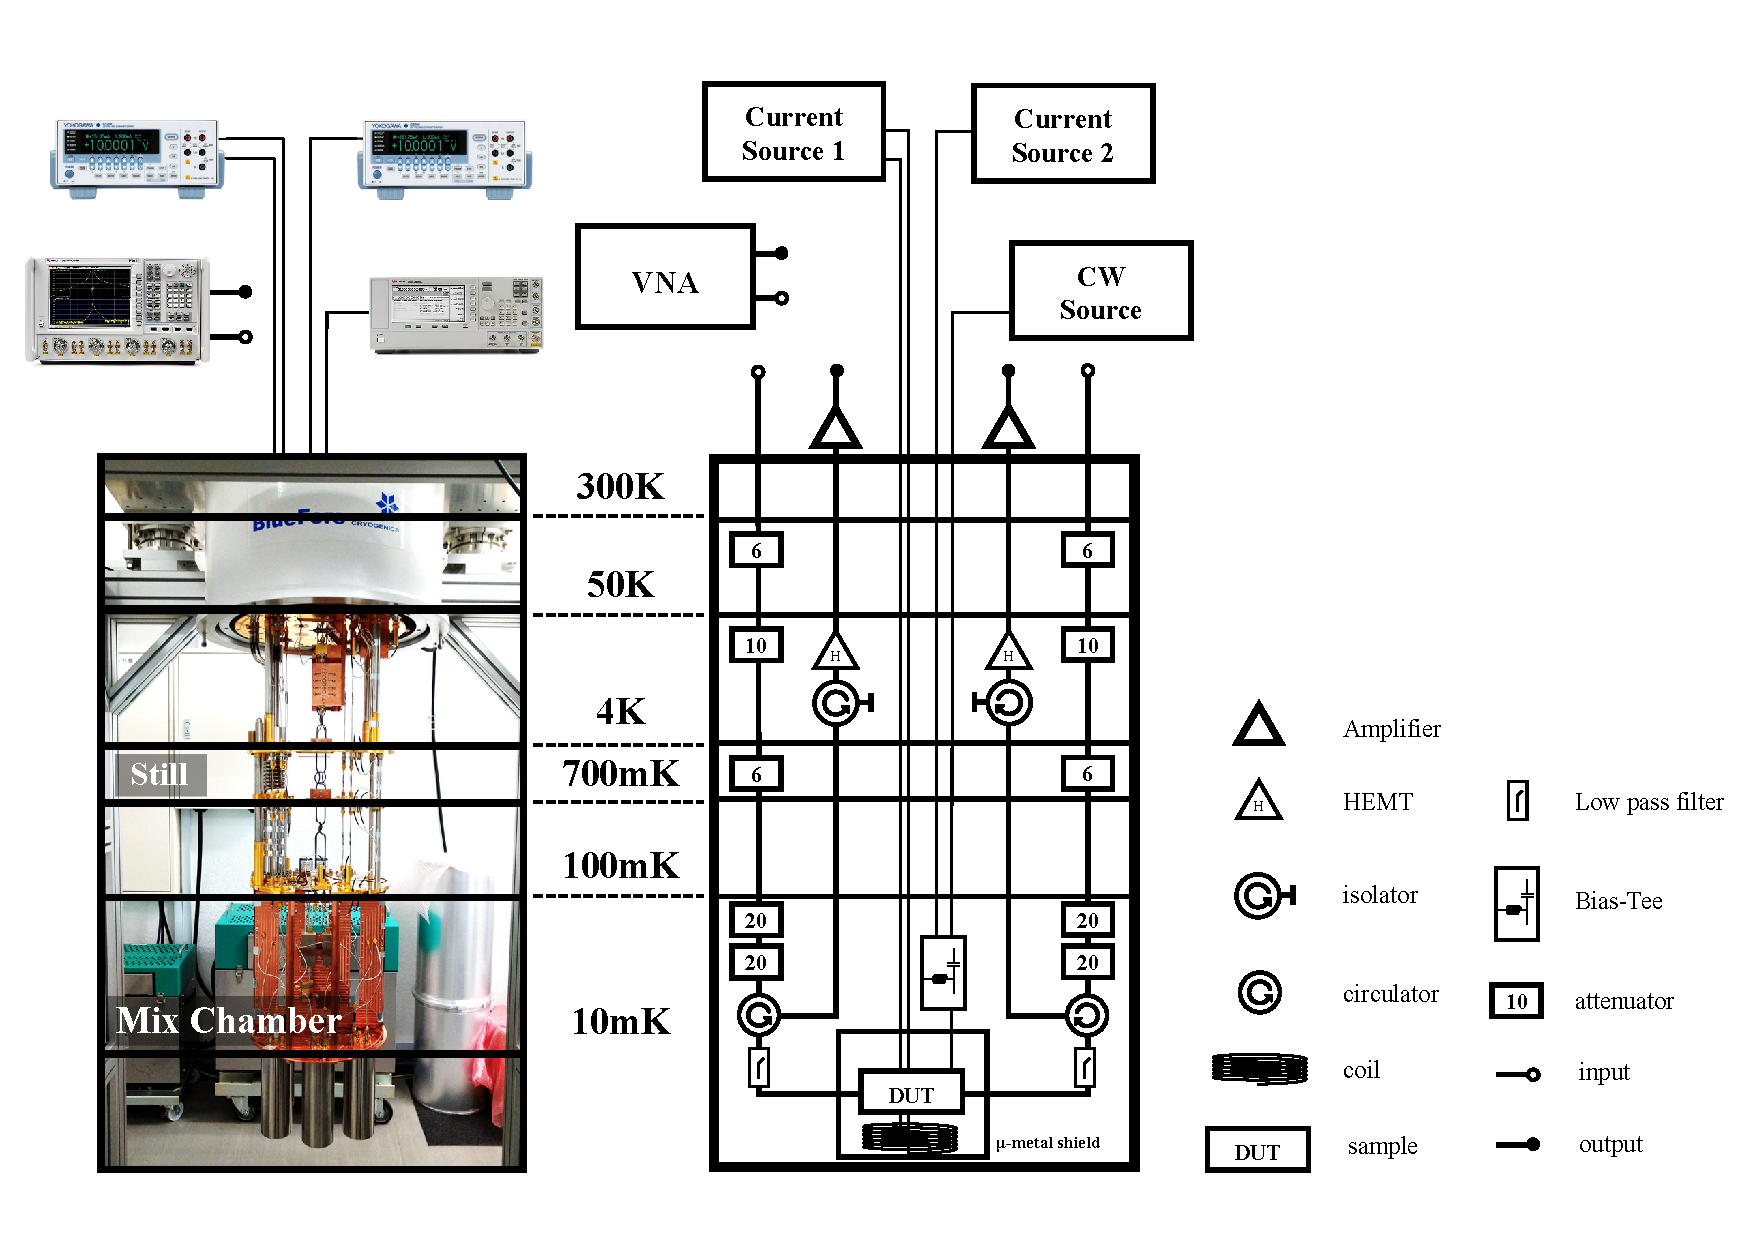
\includegraphics[width=11.5cm,angle=-90]{fridgesetup2.pdf}
        \caption{希釈冷凍機のセットアップs}
    \end{figure}


\chapter{考察}
    \begin{abstract}
        解析手法の説明と測定結果からいえる結合性能について言及
    \end{abstract}
    \section{結合性能}

\section{結合振動子の物理}



\chapter{結論}
    \begin{abstract}
        結合素子として使えるのかどうか総論
    \end{abstract}
    \section{解析を終えて}


\chapter{展望}
    \begin{abstract}
        今後改善可能性のある部分について言及
    \end{abstract}
    \section{今後の展望}


\chapter{謝辞}
    \begin{abstract}
        謝辞
    \end{abstract}
    \section*{謝辞}
本研究を進めるにあたってお世話になった方々にこの場を借りて御礼申し上げます。
指導教員の蔡教授には日々の研究指導並びに充実した研究環境を与えてくださったこと厚く感謝しております。誠にありがとうございました。
共同研究者の向井寛人氏、朝永顕成氏、伊藤輝氏には日々の充実した議論をしていただき研究を推し進めることができました。ありがとうございました。
特に、朝永顕成氏には研究室配属から卒業までサンプル作成及び研究活動において大変サポートしていただきました。ありがとうございました。

最後に日々活発な議論をしてくださった蔡研究室の皆様、研究活動をサポートしてくださった皆様に感謝申し上げます。ありがとうございました。


This paper is based on results obtained from a project commissioned by the New Energy and
Industrial Technology Development Organization (NEDO). Supports from CREST, JST (Grant
No. JPMJCR1676), and ImPACT Program of Council for Science, Technology and Innovation
(Cabinet Office, Government of Japan) are also appreciated.

\chapter{補足}
    \begin{abstract}
        本文に直接記載すると煩雑になりがちだが重要な計算をここに記す。
    \end{abstract}
    \section{ハミルトニアンの基底変換}
ここでは、Hamiltonianのs変換を行う。
\begin{equation}
    \hat{\mathcal{H}}=\hbar\left(\hat{a}^{\dagger }\ \hat{b}^{\dagger }\right)\left(\begin{array}{cc}
    \tilde{\omega}_{a} & g(\Phi ) \\
    g(\Phi ) & \hat{\omega}_{b}
    \end{array}\right)\left(\begin{array}{l}
    \hat{a} \\
    \hat{b}
    \end{array}\right)
\end{equation}
\begin{equation}
    = \hbar \hat{\omega}_{a} \hat{a}^{\dagger} \hat{a}+\hbar \hat{\omega}_{b} \hat{b}^{\dagger} \hat{b}+\hbar g(\Phi)\left(\hat{a}^{\dagger}\hat{b}+\hat{a} \vec{b}^{+}\right)
\end{equation}
\begin{equation}
    \hat{c}_{\pm}=\frac{\hat{a} \pm \hat{b}}{\sqrt{2}} \quad \hat{c}_{+}^{\dagger}=\frac{\hat{a}^{\dagger} \pm \hat{b}^{\dagger}}{\sqrt{2}}
\end{equation}
\begin{equation}
    \hat{a}^{\dagger}=\frac{\hat{c}_{+}^{\dagger}+\hat{c}_{-}^{\dagger}}{\sqrt{2}} \quad \hat{b}=\frac{\hat{c}_{+}^{\dagger}-\hat{c}_{-}^{\dagger}}{\sqrt{2}}
\end{equation}
\begin{equation}
    \hat{a}=\frac{\hat{c}_{+}+\hat{c}}{\sqrt{2}} \quad \hat{b}=\frac{\hat{c}_{+}-\hat{c}_{-}}{\sqrt{2}}
\end{equation}
\begin{equation}
    \hat{a}^{\dagger} \hat{a}=\frac{1}{2}\left(\hat{c}_{+}^{\dagger}+\hat{c}_{-}^{+}\right)\left(\hat{c}_{t}+\hat{c}_{-}\right) \quad \hat{a}^{\dagger} \hat{b}=\frac{1}{2}\left(\hat{c}_{t}^{+}+\hat{c}_{-}^{+}\right)\left(\hat{c}_{+}-\hat{c}_{-}\right)
\end{equation}
\begin{equation}
    \hat{b} \hat{b}=\frac{1}{2}\left(\hat{c}_{t}+\hat{c}_{-}^{+}\right)\left(\hat{c}_{+}-\hat{c}_{-}\right) \quad \hat{a} \hat{b}^{\dagger}-\frac{1}{2}\left(\hat{c}_{t}+\hat{c}_{-}\right)\left(\hat{c}_{t}^{+}-\hat{c}_{-}^{+}\right)
\end{equation}
\begin{equation}
    \hat{a}^{\dagger} \hat{a}=\frac{1}{2}\left[\hat{c}_{t}^{+} \hat{c}_{+}+\hat{c}_{t}^{+} \hat{c}+\hat{c}_{-}^{+} \hat{c}_{t}+\hat{c}_{-}^{+} \hat{c}_{-}\right]
\end{equation}
\begin{equation}
    \hat{b}^{\dagger} \hat{b}=\frac{1}{2}\left[\hat{c}_{t}^{*} \hat{c}_{t}-\hat{c}_{t}^{n} \hat{c}-\hat{c}_{-}^{+} \hat{c}_{t}+\hat{c}_{-}^{+} \hat{c}-\right]
\end{equation}
\begin{equation}
    \hat{a}^{\dagger} \hat{b}=\frac{1}{2}\left[\dot{c}+\hat{c}_{t}-\hat{c}_{t} \hat{c}_{-}+\hat{c}_{-}^{+} \hat{c}_{t}-\hat{c}_{-}^{\prime} \hat{c}_{-}\right]
\end{equation}
\begin{equation}
    \hat{a} \hat{b}^{\dagger}=\frac{1}{2}\left[\hat{c}_{+} \hat{c}_{+}^{4}-\hat{c}_{+} \hat{c} \pm+\hat{c}-\hat{c}_{+}^{2}-\hat{c}-\hat{c}_{-}\right]
\end{equation}
\begin{equation}
    \hat{H}=\frac{\hbar}{2} \hat{w}_{a}\left[\hat{c}_{t}^{+} \hat{c}_{+}+\hat{c}_{t}^{+} \hat{c}+\hat{c}_{-}^{+} \hat{c}_{t}+\hat{c}_{-}^{+} \hat{c}_{-}\right]
\end{equation}
\begin{equation}
    +\frac{\hbar}{2} \hat{\omega}_{b}\left[\hat{c}_{+}^{+} \hat{c}_{+}-\hat{c}_{+}^{+} \hat{c}_{-}-\hat{c}_{-}^{+} \hat{c}_{+}+\hat{c}_{-}^{+} \hat{c}_{-}\right]
\end{equation}
\begin{equation}
    +\frac{\hbar}{2} g\left[2 \hat{c}+\hat{c}_{+}-2 \hat{c}_{-} \hat{c}\right]
\end{equation}
\begin{equation}
    \hat{H}=\frac{\hbar}{2}\left(\hat{\omega}_{a}+\hat{\omega}_{b}+2 g(\Phi)\right) \hat{c}_{t}^{+} \hat{c}_{+}+\frac{\hbar}{2}\left(\hat{w} a+\hat{w}_{b}-2 g(\Phi)\right) \hat{c}_{-}^{+} \hat{c}_{-}
\end{equation}
\begin{equation}
    +\frac{\hbar}{2} A\left(\hat{w}_{a}-\hat{w}_{b}\right)\left(\hat{c}_{t}+\hat{c}_{-}+\hat{c}_{+} \hat{c}_{-}\right)
\end{equation}
\begin{equation}
    \omega_{a}+\bar{c}_{b}+2 g(\Phi)=\Omega+
\end{equation}
\begin{equation}
    \omega_{a}+\bar{c}_{b}-2 g(\Phi)=\Omega-
\end{equation}
\begin{equation}
    \hat{\omega}_{a}-\hat{w}_{b}=\Delta
\end{equation}
\begin{equation}
    \hat{H}=\frac{\hbar}{2} \Omega+\hat{c}+\hat{c}+\frac{\hbar}{2} \Omega-\hat{c} \pm \hat{c}+\frac{\hbar}{2} \Delta\left(\hat{c}+\hat{c}+\hat{c}_{+} \hat{c}_{-}^{+}\right)
\end{equation}
\begin{equation}
    -\frac{\hbar}{2}\left(\begin{array}{cc}
    \hat{c}_{+} & \hat{c} \pm
    \end{array}\right)\left(\begin{array}{cc}
    \Omega_{1} & \Delta \\
    2 & \Omega_{2}
    \end{array}\right)\left(\begin{array}{l}
    \hat{c}_{+} \\
    \hat{c}_{-}
    \end{array}\right)
\end{equation}

\section{rf-SQUIDの相互インダクタンス}
dc-SQUIDのインダクタンスは
\begin{equation}
    L_{s}(\Phi)=\frac{\Phi_0}{4\pi I_{c}|{\cos({\phi_{-}^{min}(\Phi_{ext})}})|}
\end{equation}
と記述することができる。
\begin{equation}
    \Phi=\Phi_{ext}+L_{loop}
\end{equation}
\begin{equation}
    \beta_{dc}=\frac{2\pi L_{loop} I_{c}}{\Phi_{0}}
\end{equation}
とすると。
\section{インターデジタルキャパシタンス}
インターデジタルキャパシタンスとは図中の共振器の櫛状になっている部分の構造である。
\begin{figure}[H]
    \label{le}
    \centering
    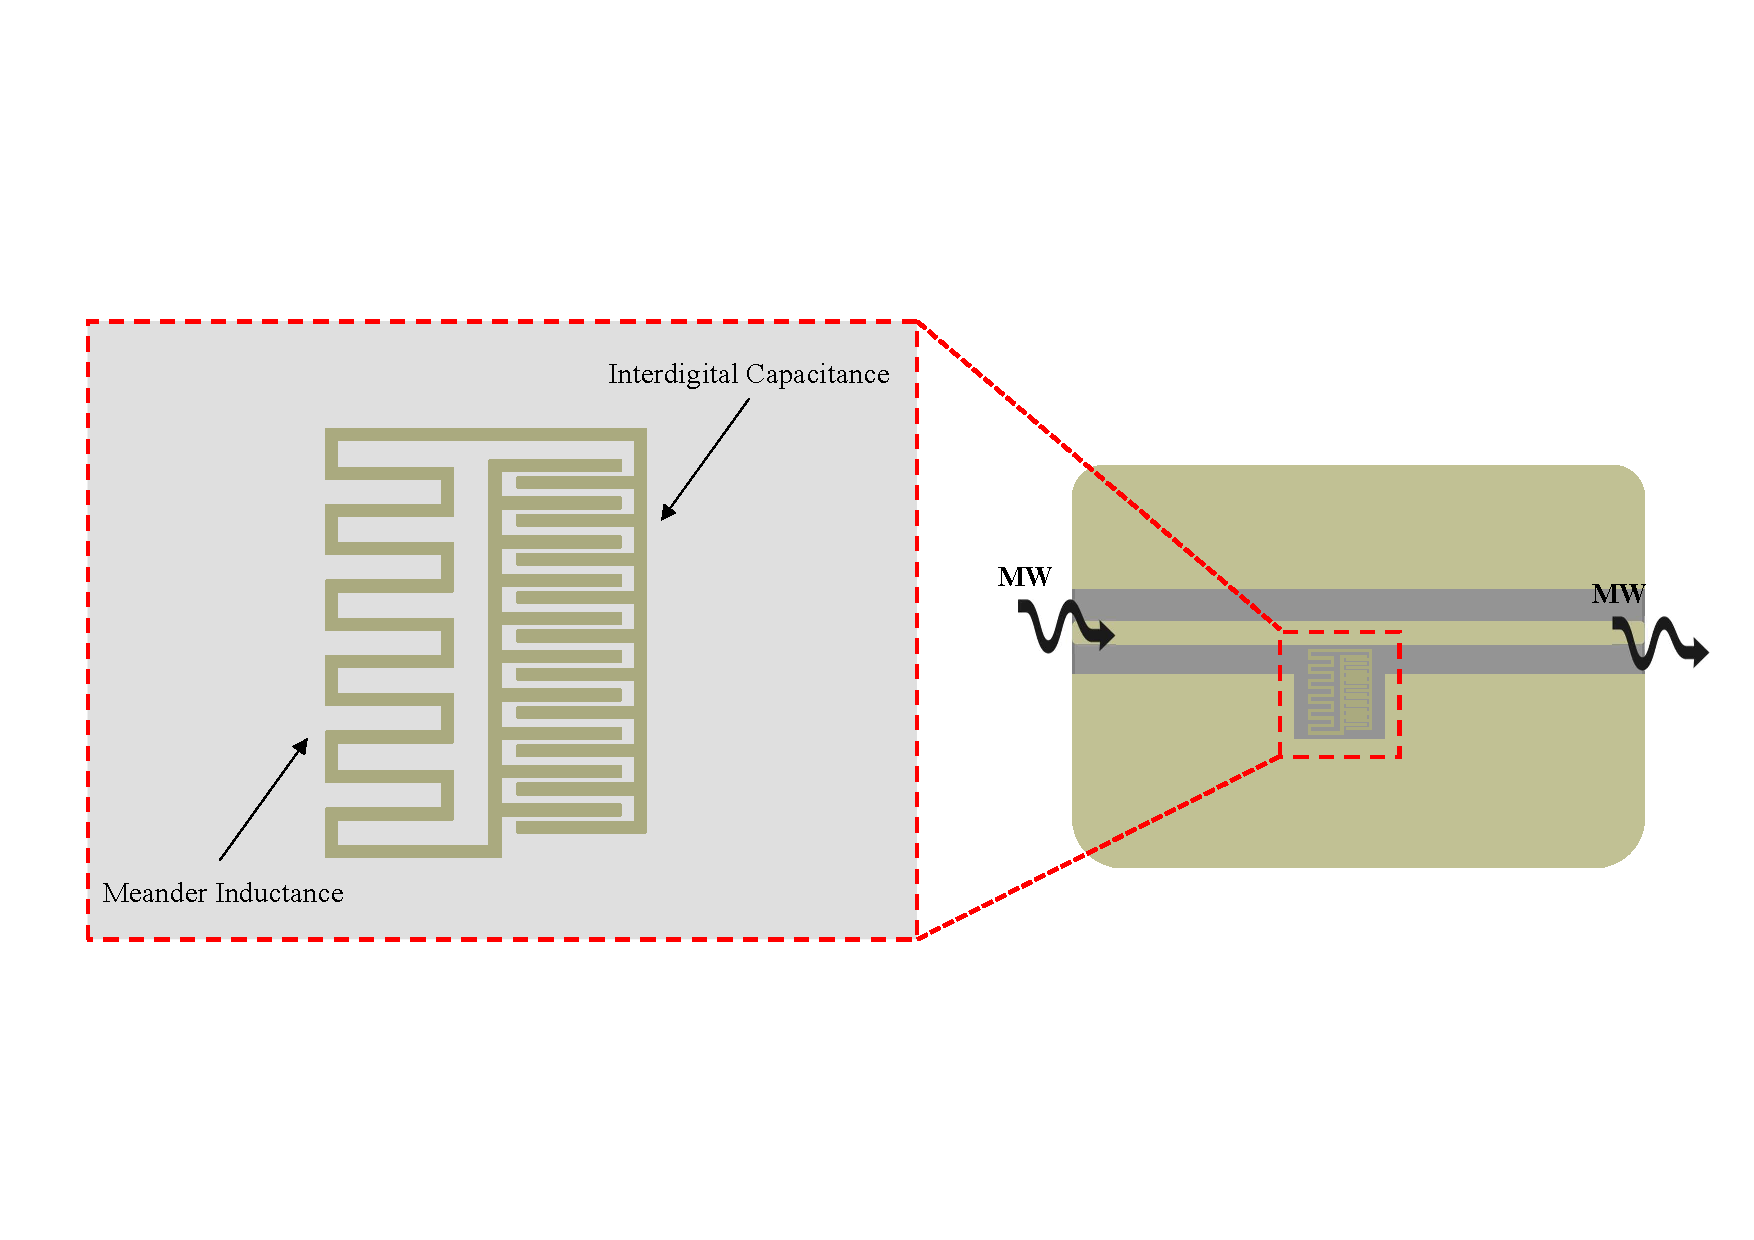
\includegraphics[width=16cm]{lumpedelement.pdf}
    \caption{準集中定数型共振器(再掲)}
\end{figure}
この構造により、電極同士の表面積を上げることでキャパシタンスを増幅することができる。ここではインターデジタルキャパシタンスの計算方法について解説を行う。また、ここで解説するインターデジタルキャパシタンスの計算方法は櫛の数が2本以上のケースである。\cite*{Gevorgian1996,Dib2005,Dib2001ComprehensiveSO}
\begin{figure}[H]
    \centering
    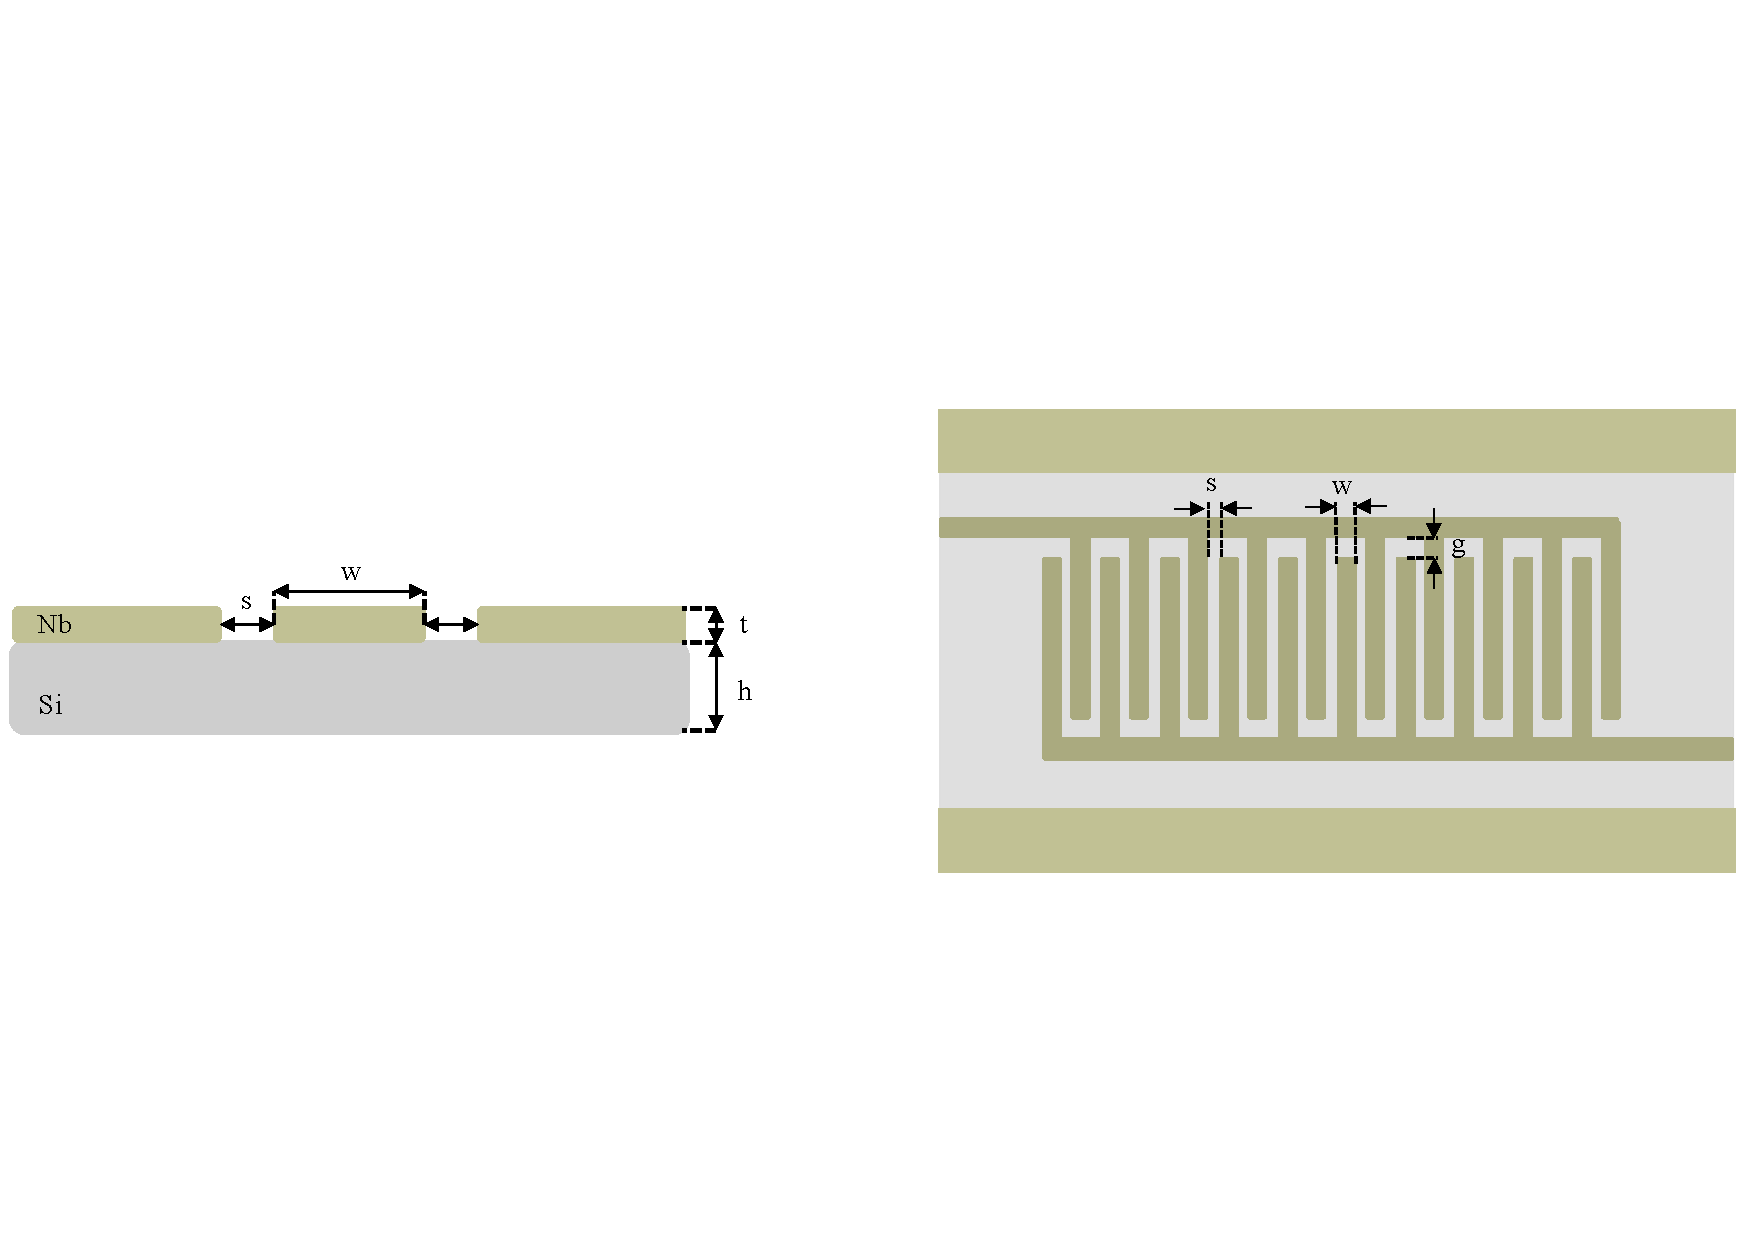
\includegraphics[width=14cm]{IDC2.pdf}
    \caption{インターデジタルキャパシタンス}
\end{figure}
式中の文字は上記の図中のパラメータに対応している。
まず線路の幅wは導体の厚さを含めた実行幅$w_eff$へと変換を行う。\cite*{Gevorgian1996}
\begin{equation}
    W_{e f f}=W+\frac{t}{\pi}\left[1+\ln \left(\frac{4 \pi W}{t}\right)\right]
\end{equation}
ここで相対する導体間のキャパシタンスをCsとする。
キャパシタンスCsを構成するのは櫛が3本であることを想定したキャパシタンスC3、櫛の本数Nに相当するキャパシタンス開放状態になっている最両端の櫛のキャパシタンスCendの3つである。
\begin{equation}
    C_{s}=C_{3}+C_{N}+C_{\text { end }}
\end{equation}
それぞれのキャパシタンスはコンフォーマルマッピングを用いて解析的に求めることが可能である。それぞれの値を求めるにはまずC3について
\begin{equation}
    C_{3}=4 \varepsilon_{0} \varepsilon_{e} \frac{K\left(k_{1}\right)}{K\left(k_{1}^{\prime}\right)} L
\end{equation}\begin{equation}
    \varepsilon_{e}=1+q_{1} \frac{\varepsilon_{r}-1}{2}
\end{equation}
\begin{equation}
        q_{1}=\frac{K\left(k_{1}^{\prime}\right)}{K\left(k_{1}\right)} \frac{K\left(k_{2}\right)}{K\left(k_{2}^{\prime}\right)}
\end{equation}
\begin{equation}
    k_{1}=\frac{W}{W+2 S} \sqrt{\frac{1-\left[\frac{W+2 S}{3 W+2 S}\right]^{2}}{1-\left[\frac{W}{3 W+2 S}\right]^{2}}}
\end{equation}
\begin{equation}
    \begin{aligned}
    k_{2}=& \frac{\sinh \left(\frac{\pi W}{4 h}\right)}{\sinh \left(\frac{\pi(W+2 S)}{4 h}\right)} 
    & \sqrt{\frac{\sinh ^{2}\left(\frac{\pi(3 W+2 S)}{4 h}\right)-\sinh ^{2}\left(\frac{\pi(W+2 S)}{4 h}\right)}{\sinh ^{2}\left(\frac{\pi(3 W+2 S)}{4 h}\right)-\sinh ^{2}\left(\frac{\pi W}{4 h}\right)}}
    \end{aligned}
\end{equation}
同様にしてCNについて求めると
\begin{equation}
    C_{N}=(N-3) \varepsilon_{0} \varepsilon_{N} \frac{K\left(k_{3}\right)}{K\left(k_{3}^{\prime}\right)} L
\end{equation}
\begin{equation}
    \varepsilon_{N}=1+q_{N} \frac{\varepsilon_{r}-1}{2}
\end{equation}
\begin{equation}
    q_{N}=\frac{K\left(k_{3}^{\prime}\right)}{K\left(k_{3}\right)} \frac{K\left(k_{4}\right)}{K\left(k_{4}^{\prime}\right)},
\end{equation}
\begin{equation}
    k_{3}=\frac{W}{W+S},
\end{equation}
\begin{equation}
    \begin{aligned}
    k_{4}=& \frac{\sinh \left(\frac{\pi W}{4 h}\right)}{\sinh \left(\frac{\pi(W+ S)}{4 h}\right)} 
    & \sqrt{\frac{\sinh ^{2}\left(\frac{\pi(W+S)}{4 h}\right)+\sinh ^{2}\left(\frac{\pi(W+ S)}{4 h}\right)}{\cosh ^{2}\left(\frac{\pi(W)}{4 h}\right)-\sinh ^{2}\left(\frac{\pi (W+S)}{4 h}\right)}}
    \end{aligned}
\end{equation}
として求まる。最後にCendについて、この計算を行う上で主に参考にしている論文\cite*{Dib2005}ではCendの計算について\cite*{Dib2001ComprehensiveSO}中の式
\begin{equation}
    C_{o c}=c_{e f f} C_{o e}\left(\epsilon_{r}=1\right)
\end{equation}
\begin{equation}
    \label{Cend}
    C_{\alpha c}\left(c_{r}=1\right)=\frac{c_{0}}{\pi}\left[\frac{1}{g^{2}} f_{s}(g, W+S, 0)+\frac{1}{W^{2}} f_{0}(W, S, 0)\right]
\end{equation}
\begin{equation}
    \label{fs}
    \begin{aligned}
    f_{s}(a, b, c) &=\frac{4}{3} c^{3}+f(a, c)+f(b, c)-4 a b c \tan ^{-1}\left(\frac{a b}{c \tau}\right)-\frac{2}{3}\left(b^{2}-2 c^{2}+a^{2}\right) \tau \\
    &+\left(a^{2}-c^{2}\right) b \ln \left(\frac{\tau+b}{\tau-b}\right)+\left(b^{2}-c^{2}\right) a \ln \left(\frac{\tau+a}{\tau-a}\right)
    \end{aligned}
\end{equation}
\begin{equation}
    \label{f0}
    f_{0}(a, b, c) =\frac{4}{3} c^{3}+f(a, c)+f(a+b, c)-\frac{1}{2} f(b+2 a, c)-\frac{1}{2} f(b, c)
\end{equation}
\begin{equation}
    \label{fx}
    f(x, y) =\frac{2}{3}\left(x^{2}-2 y^{2}\right) \sqrt{x^{2}+y^{2}}+y^{2} x \ln \left(\frac{\sqrt{x^{2}+y^{2}}+x}{\sqrt{x^{2}+y^{2}}-x}\right)
\end{equation}
を使用したと記述されているが式\ref*{fx}の第2項目は不適切であるため、本稿では含めずに計算した。というのも式\ref*{fx}が使用されている式\ref{Cend,fs,f0}に注目すると式\label{fx}中の$y$は常にゼロであり、第2項目は2乗でゼロに収束する。よって2項目は計算に含まれないことになる。よって計算には以下
\begin{equation}
    \label{fx_re}
    f(x, y)_{revised} =\frac{2}{3}\left(x^{2}-2 y^{2}\right) \sqrt{x^{2}+y^{2}}
\end{equation}
をもちいた。
以上の計算式を用いてインターデジタルキャパシタンスの値を見積もることができる。
ここではさらに本稿で使用したパラメータを用いて櫛の本数Nに対してキャパシタンスの値がどれだけ変化するのか、また、実験結果との比較を行う。
\begin{figure}[H]
    \centering
    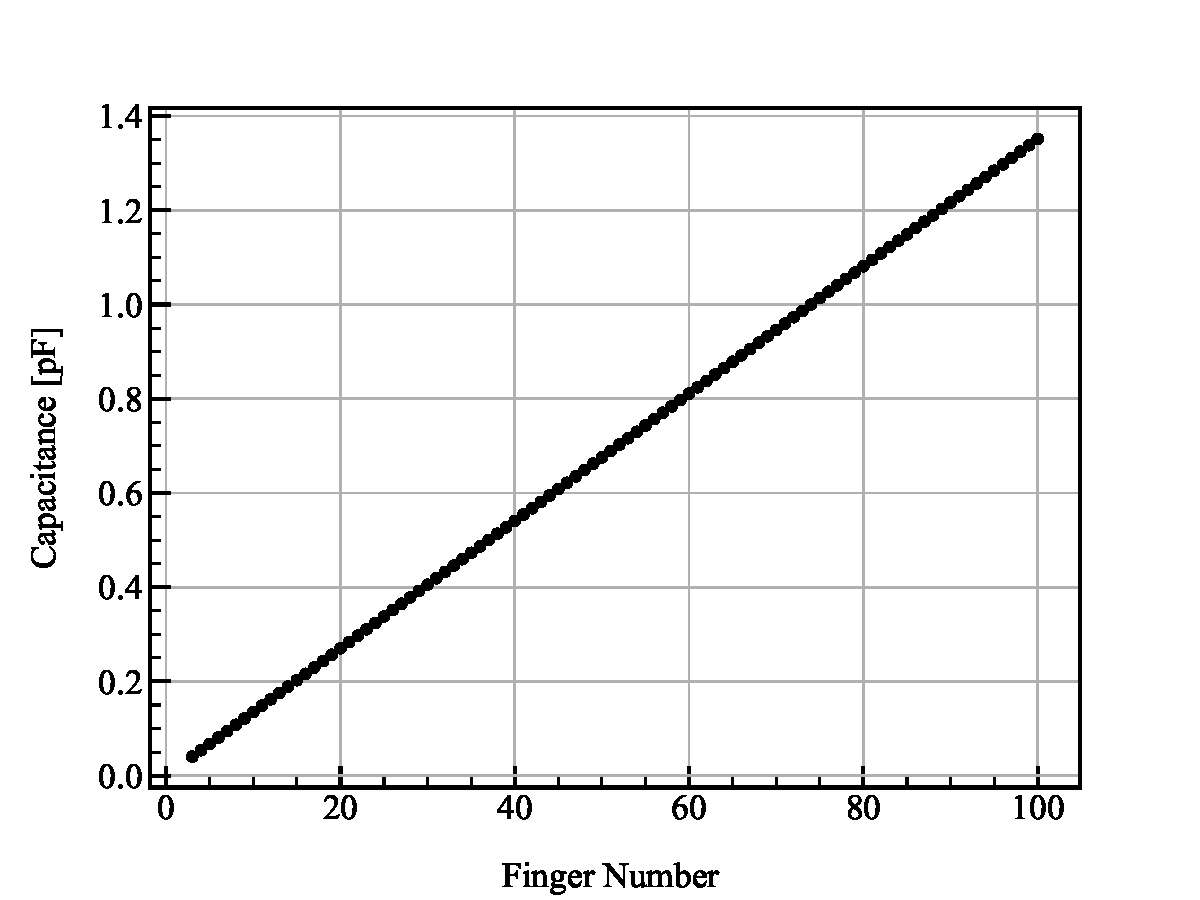
\includegraphics[width=10cm]{IDC_cal.pdf}
    \caption{キャパシタンス vs 櫛の本数}
\end{figure}
\section{ミアンダインダクタンス}
ミアンダインダクタンスとは図\ref{le}中蛇行した構造を持ったインダクタのことを指している。蛇行させることによりサイズに対して線路長が長くなり、また、相対する相互インダクタンスによりインダクタンスの総和が増加する。ここでは本稿で用いたミアンダインダクタンスの解析的計算方法について解説する。本文中ではここで行った解析的計算の結果と電磁界シミュレーションによるミアンダインダクタンス部分の計算を比較していので参照されたい。
\begin{figure}[H]
    \label{ミアンダ}
    \centering
    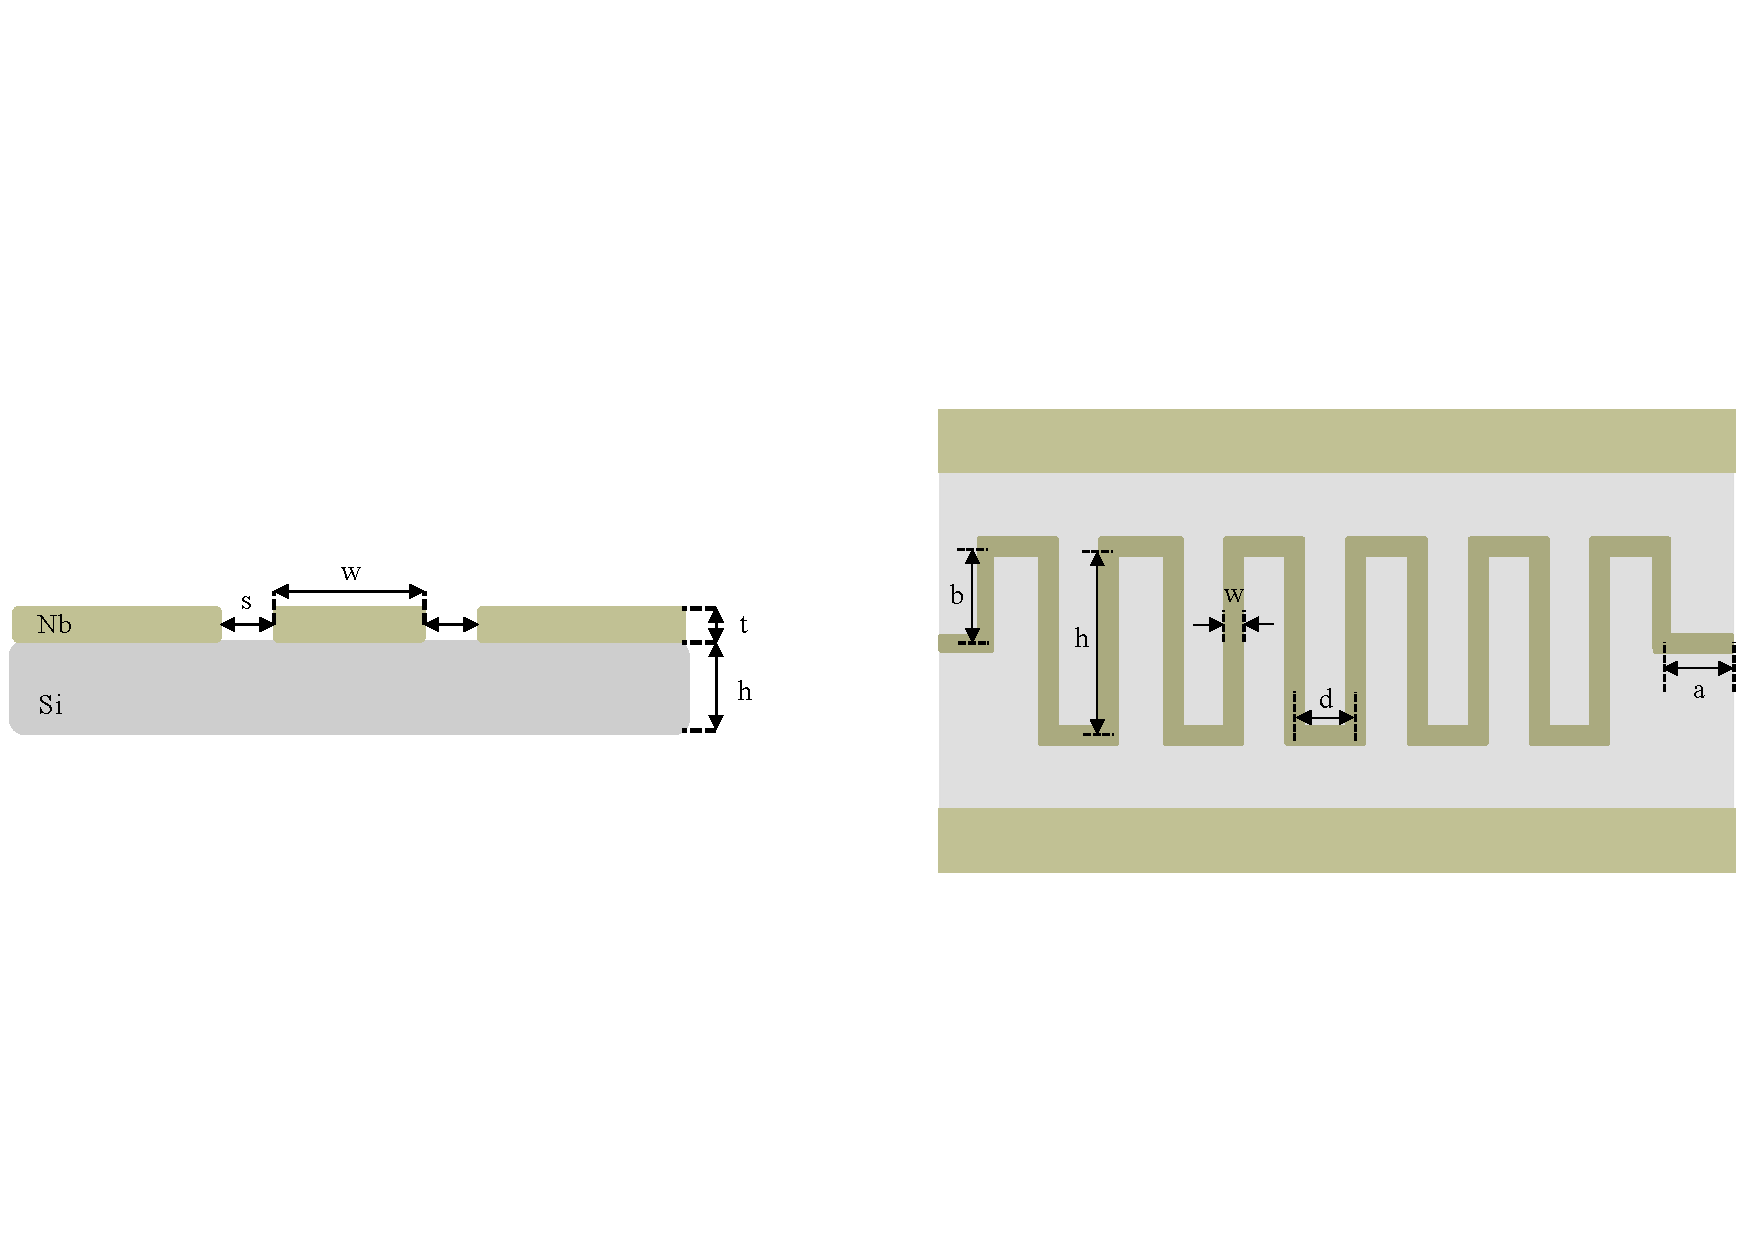
\includegraphics[width=14cm]{ミアンダ.pdf}
    \caption{ミアンダインダクタンス}
\end{figure}
以下数式は上図のパラメータに対応する。この計算に主に参考にした論文は\cite*{Stojanovic2004}である。
文献\cite*{Grover}より長方形線路の自己インダクタンスは
\begin{equation}
    L=0.002 l\{\ln [2 l /(w+t)]+0.50049+[(w+t) / 3 l]\}
\end{equation}
である。ここでwは線路幅、tは厚さ、lは線路長である。ミアンダインダクタンスの大部分を占めているのは各セグメントに於ける自己インダクタンスの総和である。すなわち、図中のパラメータによって各セグメントをラベル付けするとミアンダインダクタンス中セルフインダクタンスの寄与は
\begin{equation}
    L_{\text {selftot }}=2 \cdot L_{a}+2 \cdot L_{b}+N \cdot L_{h}+(N+1) \cdot L_{d}
\end{equation}
である。ここでNはセグメントhの本数に対応する。図\ref*{ミアンダ}ではN=10である。参考文献ではいくつかタイプミスが見受けられたため、少々煩雑ではあるが式の全文を記すこととする。
既に記した条件を前提とした上でNがの偶奇で計算は異なる。
\begin{figure}[H]
    \label{偶奇}
    \centering
    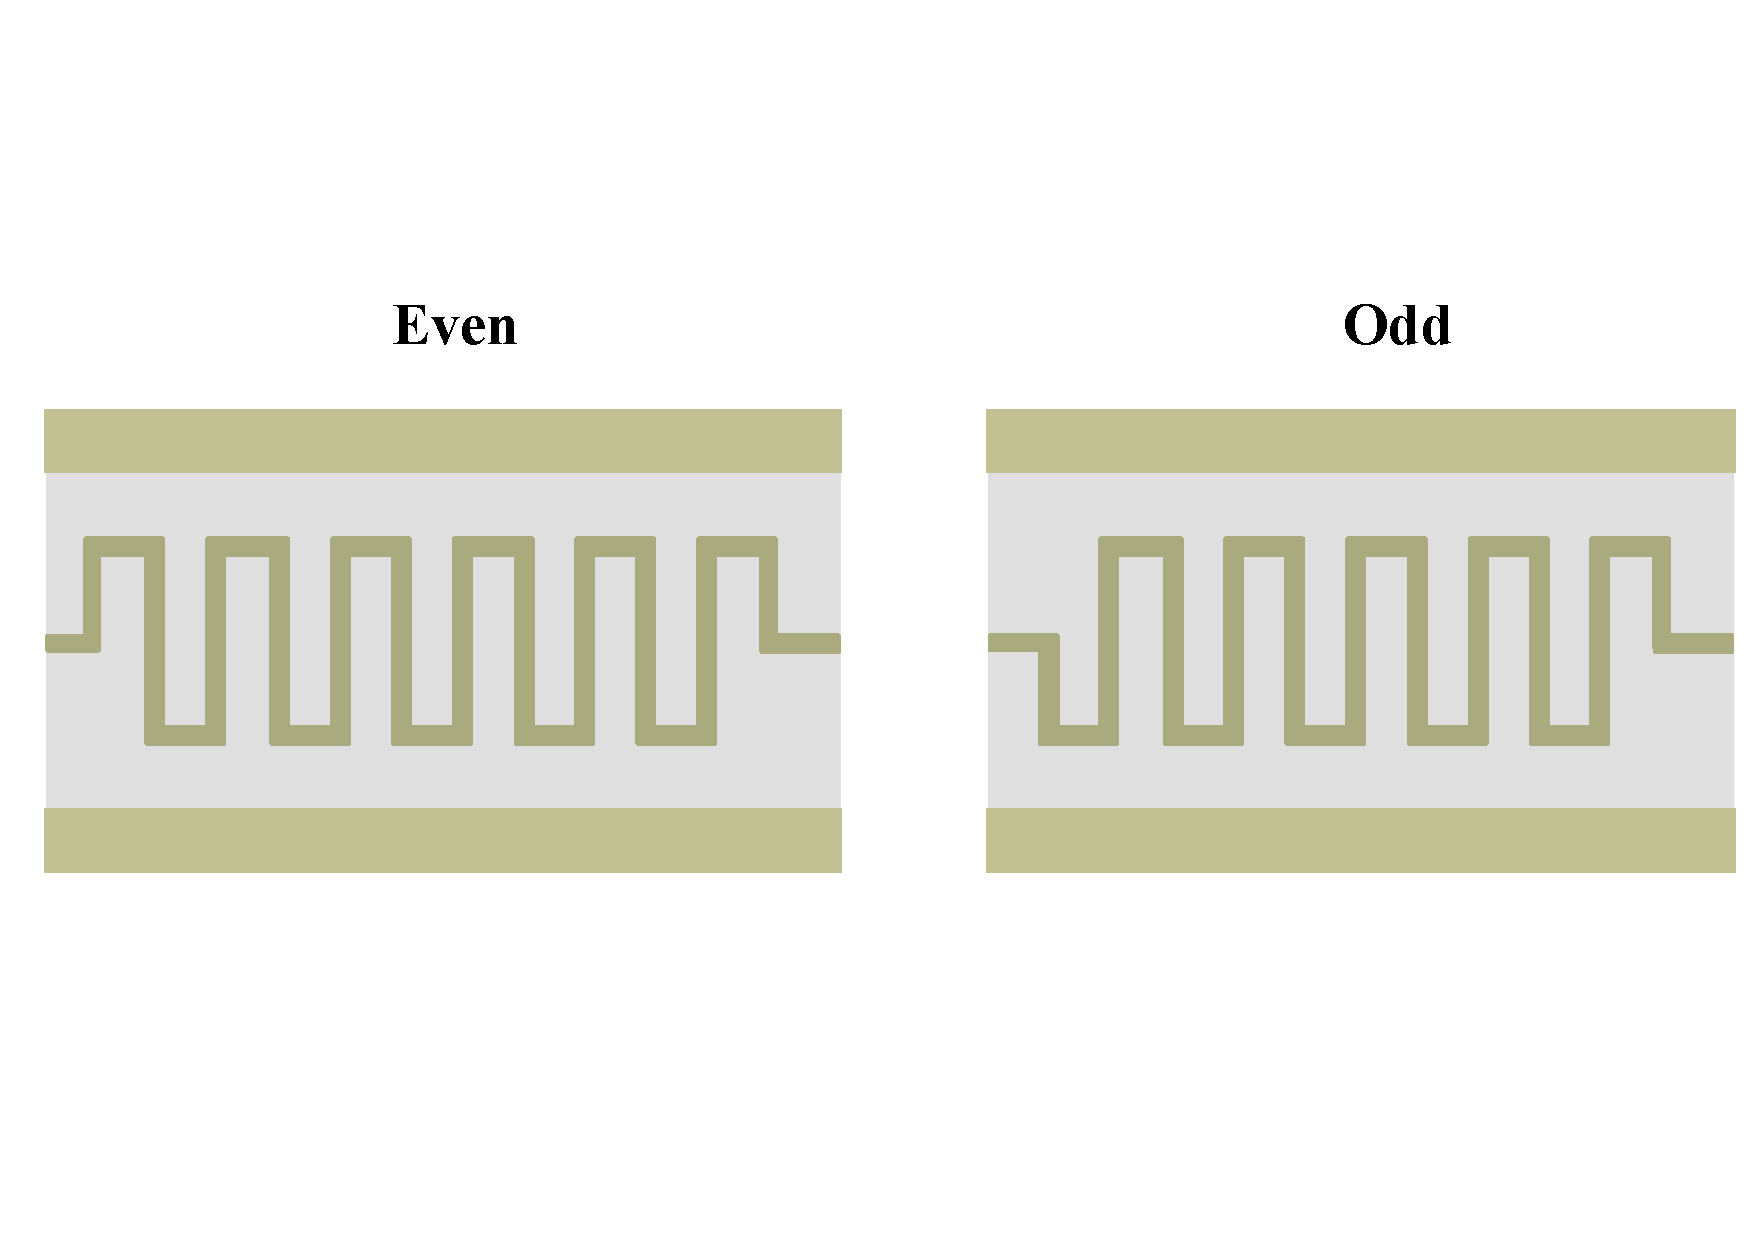
\includegraphics[width=14cm]{偶奇.pdf}
    \caption{ミアンダインダクタンス}
\end{figure}
文献\cite*{Grover}に依れば相対する線路に於ける相互インダクタンスは
\begin{equation}
    M=0.002 l\left[\log _{e}\left(\frac{l}{d}+\sqrt{1+\frac{l^{2}}{d^{2}}}\right)-\sqrt{1+\frac{d^{2}}{l^{2}}}+\frac{d}{l}\right]
\end{equation}
\begin{figure}[H]
    \label{相互}
    \centering
    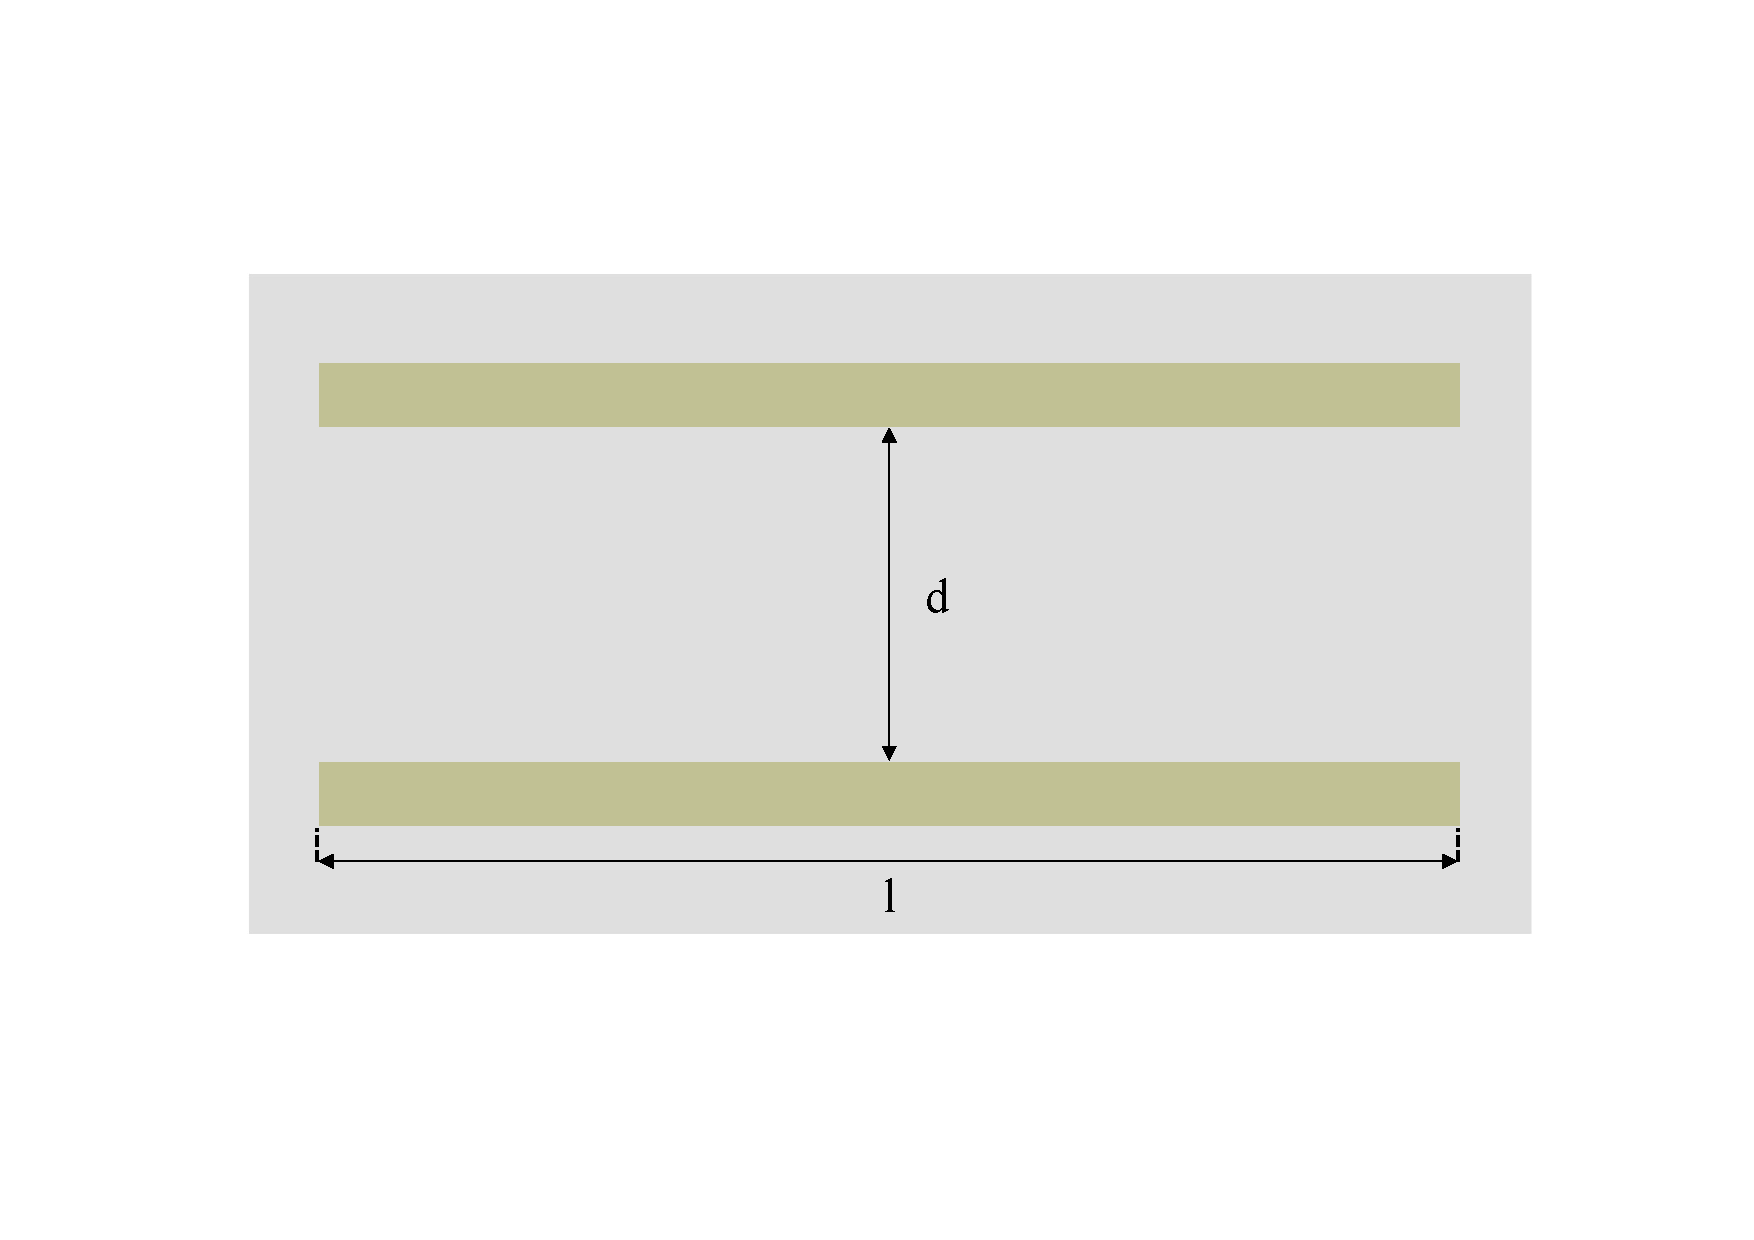
\includegraphics[width=8cm]{相互.pdf}
    \caption{2線路間に於ける相互インダクタンス}
\end{figure}
線路間の相互インダクタンスは配置によって以下の4通りのケースが存在する。
\begin{figure}[H]
    \centering
    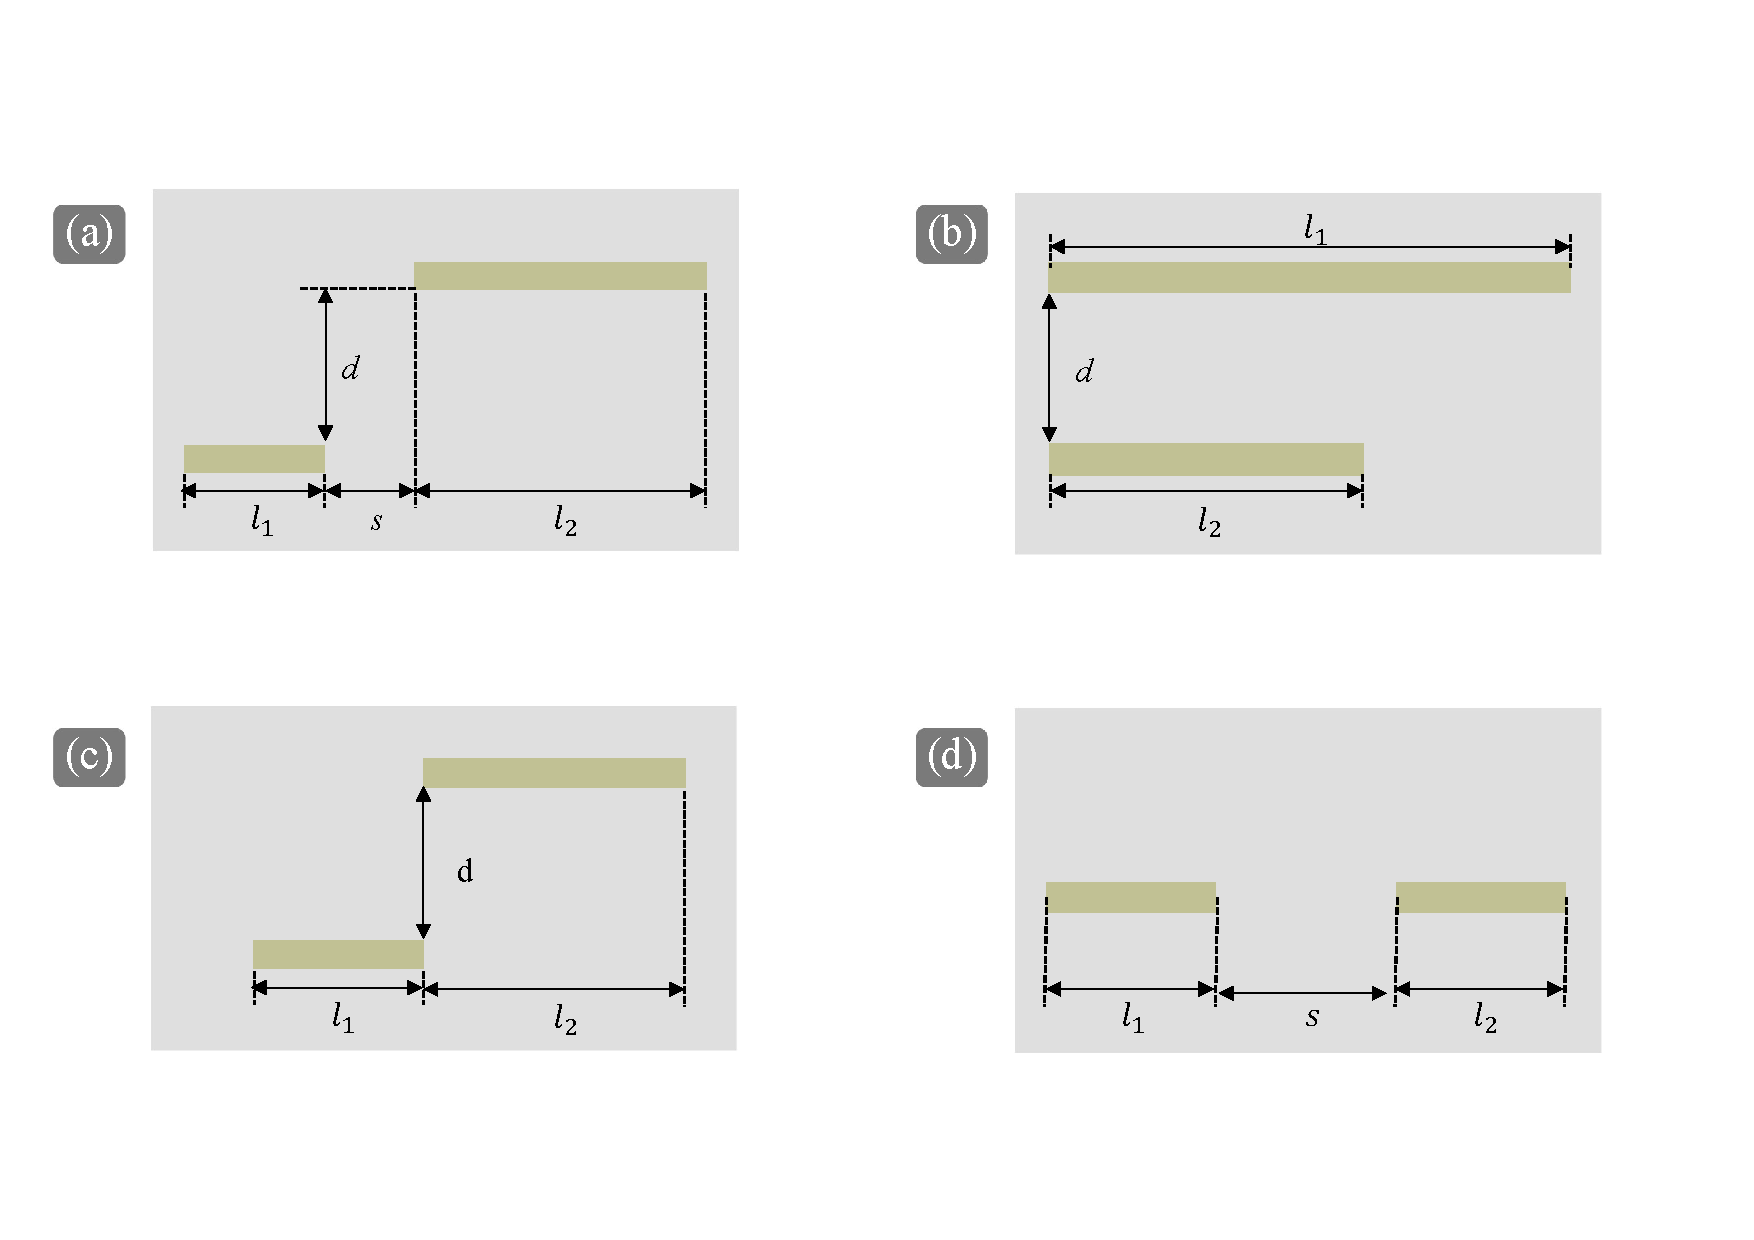
\includegraphics[width=14cm]{mutual.pdf}
    \caption{2線路間に於ける相互インダクタンス}
\end{figure}
よってそれぞれについて相互インダクタンスの関数を以下のように定義する。
\begin{equation}
    M_{a 1}\left(l_{1}, l_{2}, r, s\right)=0.5 \cdot\left[M_{c}\left(l_{1}+l_{2}+s, r\right)+M_{c}(s, r)-M_{c}\left(l_{1}+s, r\right)-M_{c}\left(l_{2}+s, r\right)\right]
\end{equation}
\begin{equation}
    M_{a 2}\left(l_{1}, l_{2}, r\right)=0.5 \cdot\left[M_{c}\left(l_{1}, r\right)+M_{c}\left(l_{2}, r\right)-M_{c}\left(l_{1}-l_{2}, r\right)\right]
\end{equation}
\begin{equation}
    M_{a 3}\left(l_{1}, l_{2}, r\right)=0.5\left[M_{c}\left(l_{1}+l_{2}, r\right)-M_{c}\left(l_{1}, r\right)-M_{c}\left(l_{2}, r\right)\right]
\end{equation}
\begin{equation}
    M_{b}\left(l_{1}, l_{2}, s\right)=\frac{\infty_{0}}{4 \pi}\left[\left(l_{1}+l_{2}+s\right) \ln \left(l_{1}+l_{2}+s\right)-\left(l_{1}+s\right) \ln \left(l_{1}+s\right)-\left(l_{2}+s\right) \ln \left(l_{2}+s\right)+s \ln (s)\right]
\end{equation}

上記の4通りの方法を各セグメントに適用することでミアンダインダクタンスに存在する相互インダクタンスをすべて勘定することができる。
偶奇それぞれについて計算する相互インダクタンスは以下の7ケースである。
\begin{figure}[H]
    \centering
    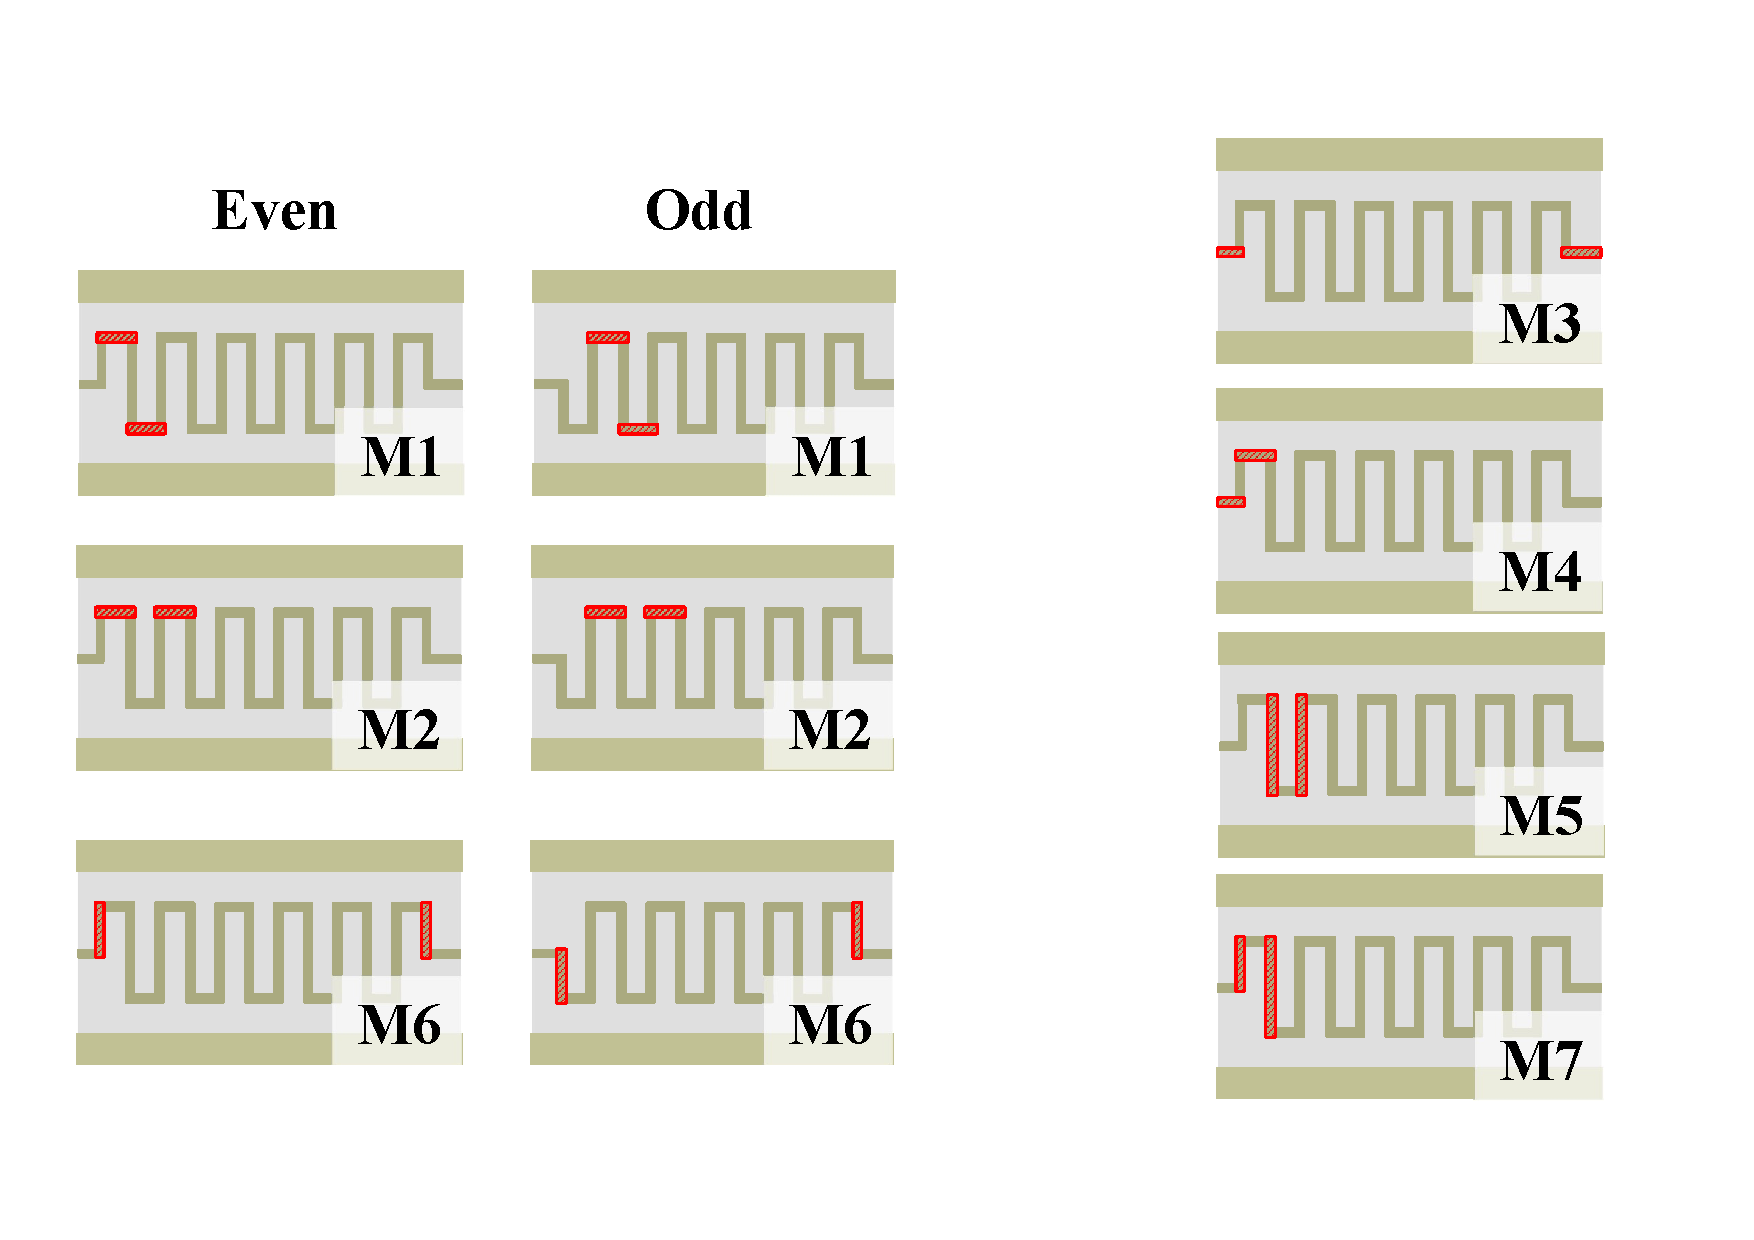
\includegraphics[width=14cm]{m2.pdf}
    \caption{セグメント別相互インダクタンス}
\end{figure}
上記のセグメント別の相互インダクタンスについて偶奇について違いあるものは
\begin{equation}
    \begin{array}{l}
    M_{1}=\sum_{i=1}^{N / 2}(2 N+4-4 i) \cdot M_{\mathrm{ul}}(d, d, h,(2 i-2) d), \text { for } N \text { even } \\
    \qquad M_{1}=\sum_{i=1}^{d}(2 N+4-4 i) \cdot M_{a 1}(d, d, h,(2 i-2) d), \text { for } N \text { odd }
    \end{array}
\end{equation}
\begin{equation}
    \begin{aligned}
    M_{2} &=\sum_{i=1}^{N / 2}(2 N+2-4 i) \cdot M_{b}(d, d,(2 i-1) d), \text { for } N \text { even } \\
    M_{2}=&\sum_{(N-1) / 2}^{\infty}(2 N+2-4 i) \cdot M_{b}(d, d,(2 i-1) d), \text { for } N \text { odd }
    \end{aligned}
\end{equation}
\begin{equation}
    \begin{aligned}
    M_{6}&=-2 \cdot M_{c}(b,(N+1) d), \text { for } N \text { even }\\
    M_{6}&=+2 \cdot M_{a 3}(b, b,(N+1) d), \text { for } N \text { odd }
    \end{aligned}
\end{equation}
また、偶奇の違いがないものについて
\begin{equation}
    M_{3}=2 \cdot M_{b}(a, a,(N+1) d)
\end{equation}
\begin{equation}
    M_{4}=\sum_{i=0}^{N} 4 \cdot M_{a 1}(a, d, b, i d)
\end{equation}
\begin{equation}
    M_{5}=\sum_{i=0}^{N-1}(-1)^{i} \cdot 2 \cdot(N-1) \cdot M_{c}(h, t d)
\end{equation}
\begin{equation}
    M_{7}=\sum_{i=0}^{N}(-1)^{i} \cdot 4 \cdot M_{a 2}\left(b_{2} h, i d\right)
\end{equation}
となる。それぞれについて各セグメントの総和
\begin{equation}
    M_{\text {tot }}=M_{1}+M_{2}+M_{3}+M_{4}+M_{5}+M_{6}+M_{7}
\end{equation}
によってミアンダインダクタンスに於ける相互インダクタンスを見積もることができる。これについて自己インダクタンスを足し合わせたもの
\begin{equation}
    L_{\text {tot }}=L_{\text {selftot }}+M_{\text {tot }}
\end{equation}
がミアンダインダクタンスとなる。ただし、本稿では線路として極低温下にある超伝導微細薄膜を用いているため線路長分のカイネティックインダクタンスを考慮する必要がある。


\section{マスター方程式}
\section{2点相関関数}
時間に依存する物理量Aについてある時間tと



%\bibliographystyle{}
\addcontentsline{toc}{chapter}{参考文献}
\printbibliography[title=参考文献]
\end{document}
